%
%This Skeleton for Master's Thesis reports is written by
%Jonas Birme during his work with his MT-report in 2004.
%Jonas is a former student and Assistant at Computing Science, UmU.
%Jonas is also the author of the documentclass thesis_report.cls
%Both these files have been modified and extended by Per Lindstr�m at Comp. Sc., UmU
%in December 2004.
%
\documentclass[a4paper]{thesis_report}
\usepackage{url}
\usepackage{hyperref}

\def\lt{{\sc <}}
\def\gt{{\sc >}}

\begin{document}
\pagestyle{empty}

\title{A Web-Based Environment for Learning Relational-Database Normalization}
\author{Nikolay Georgiev}
\credits{30} 
\supervisor{Stephen J. Hegner}
\examiner{Per Lindstr\"om} %Name of examiner (normally Per Lindstr�m}

\maketitle
\cleardoublepage

%%%%%%%%%%%%%%%%%%%%%%%%%%%%%%%%%%%%%%%%
%   Abstract
%%%%%%%%%%%%%%%%%%%%%%%%%%%%%%%%%%%%%%%%
\pagenumbering{roman} \setcounter{page}{1}
\pagestyle{fancy}
\begin{abstract}
Database normalization is a technique for designing relational database tables 
to minimize duplication of information in order to safeguard the database 
against certain types of logical or structural problems, namely data anomalies. 
Therefore database normalization is a central topic in database theory, and its 
correct understanding is crucial for students. Unfortunately  the subject it is 
often considered to be dry and purely theoretical and it is widely being disregarded 
by the students. A web-based learning environment is developed to give 
students an interactive hands-on experience in database normalization process. It
also provides lecturers with an easy way for creating and testing assignments 
on the subject.  
The learning environment is suitable for relational database and design and data 
management courses. 

This report describes the design and development of LDBN 
(Learn DataBase Normalization) - a reference implementation of the learning environment.
It also discuss problems that lie within educational and web-based software development.
A tutorial on the right usage of LDBN is also provided.   
%keywords (do we need them?)
%\newline
%\newline
%\textbf{Keywords:} Database Normalization, Relational Data Model, Functional Dependency, 
%Third Normal Form, Boyce-Codd Normal Form, Embedded Functional Dependencies

\end{abstract}

\cleardoublepage
\begin{spacing}{1.2}
\tableofcontents%
\cleardoublepage
\end{spacing}

\pagenumbering{arabic} \setcounter{page}{1}

\chapter{Introduction}
\label{chap:introduction}
Readers unfamiliar with the terms of relational-database normalization and 
functional dependencies can find a brief introduction on the subject in
Chapter~\ref{chap:preliminaries}. 

Due to its great importance for database applications database schema design has
attracted a lot of researchers~\cite{p1}. Relational-database normalization is a 
theoretical approach for organizing data in a database and it is very well developed, 
unfortunately, however, theory does not have much impact on practice yet~\cite{p1}.
One of the reasons for this is the lack of good tools which could aid the students 
during the learning process of relational-database normalization~\cite{p8}. 
Thus our learning environment was developed in order to give students the ability to 
easily and efficiently test
their knowledge of the different normal forms in practice. Moreover, normal forms are formal
notations, which ensure low storage cost and low update cost for databases, they are discussed
more formally in Chapter~\ref{chap:preliminaries}. The environment assists the students by 
providing them the following functionalities:

\begin{enumerate}
	\item Allow the student to specify a candidate decomposition of a given relation.
	\item Assess the correctness of the student's proposed decomposition relative to many factors; including:
		\begin{itemize}
			\item Lossless join property.
			\item Dependency preservation.
			\item Specification of keys.
			\item Correctness of the 2NF, 3NF and BCNF decompositions.
		\end{itemize}
	\item Provide students with sample decompositions when needed. 
	\item Allow users to communicate with each other via comments/posts.
\end{enumerate}

Our learning environment uses many different normalization 
algorithms for achieving the functionalities described above. 
We can divide them into two different groups:

\begin{description}
	\item[Decomposition algorithms] are used for decomposing a normalized database 
	schema into a certain normal form using functional dependencies (FDs).
	\item[Test algorithms] for testing , whether a given relational schema is 
	violating certain normal form, the lossless join property or other criteria.
\end{description}

It is very important to note that the \textit{Decomposition algorithms} are not enough for
our purposes, since they have the 
disadvantage that they could decompose a schema, which is already satisfying 
certain normal form, into a new set of relations/tables~\cite{p4}. Thus there can be many 
possible, distinct decomposition of the same schema, which all satisfy the same 
normal form~\cite{bdb4}. This is a key aspect of the relational-database normalization,
which does not allow us to simply compare the
students' solutions against solutions provided by the decomposition algorithms,
therefore we need the \textit{Test algorithms}.

Here it is worth mentioning that the normalization algorithms often require 
extensive relational algebraic backgrounds that most IS/IT students lack~\cite{p8}. This
is also an issue which our tool is trying to overcome by providing more intuitive 
way of decomposing a schema and by giving an easy way for lecturers to
teach by example and test the knowledge of their students. 

\section{Organization of This Report}
\label{sec:organization}
In the reminig sections of this chapter we are going to informally introduce 
the key features and consepsts of our web-based learning environment, 
called LDBN (Lean DataBase Normalization)~\cite{wldbn}; 
compare it with a couple of other 
available web-based database normalization tools; provide the reader with small glossary.  
The introduction of LDBN in Section~\ref{sec:introldbn} is important for the reader
in order for him/her to better understand the need and the concepts of the algorithms described in 
Chapter~\ref{chap:preliminaries}, where we also give definitions to
relational-database normalization and to the different normal forms. 
In Chapter~\ref{chap:design} we discuss some design issues regarding LDBN like 
platform choice and others. Chapter~\ref{chap:impl} provides a formal description
of our reference implementation of the learning environment. 
Chapter~\ref{chap:conclusion} shows our conclusions, and 
Appendix~\ref{chap:tutorial} contains a simple tutorial to the system.

\section{Learning Database Normalization with LDBN}
\label{sec:introldbn}
In this section we are going to briefly introduce our reference implementation
of the web-based learning environment, called LDBN.    
Figure~\ref{fig:screen01} shows an overview of the most important part of the UI - 
the \textit{Solve Assignment} view/tab. Here students can test their knowledge on 
the subject of relational-database normalization. The first thing the reader 
may notice is the fact that LDBN is running within a browser. The client-side 
of LDBN is written in JavaScript following the AJAX techniques 
(more about this in Chapter~\ref{chap:design}). 
Furthermore, LDBN is assignment driven. This means students have to first 
choose an assignemtn 
form a list with assignments, submitted by other users (lecturers). 
Such a list is shown in Figure~\ref{fig:screen02}. 
Moreover, an assignment consists of a relational-database schema in
universal-relation form (URF), i.e., all the attributes in a single relation 
and a set of FDs on the attributes. 
After an assignment has been loaded, we require the students to go through the 
following steps in LDBN:
\begin{enumerate}
	\item Determine a minimal cover of the given FDs, also known as canonical cover.
	\item Decompose the relational schema from URF into 2NF, 3NF and BCNF. 
	\item Determine a candidate key for each new relation/table. 
\end{enumerate}

\begin{figure}[h]
	\begin{center}
		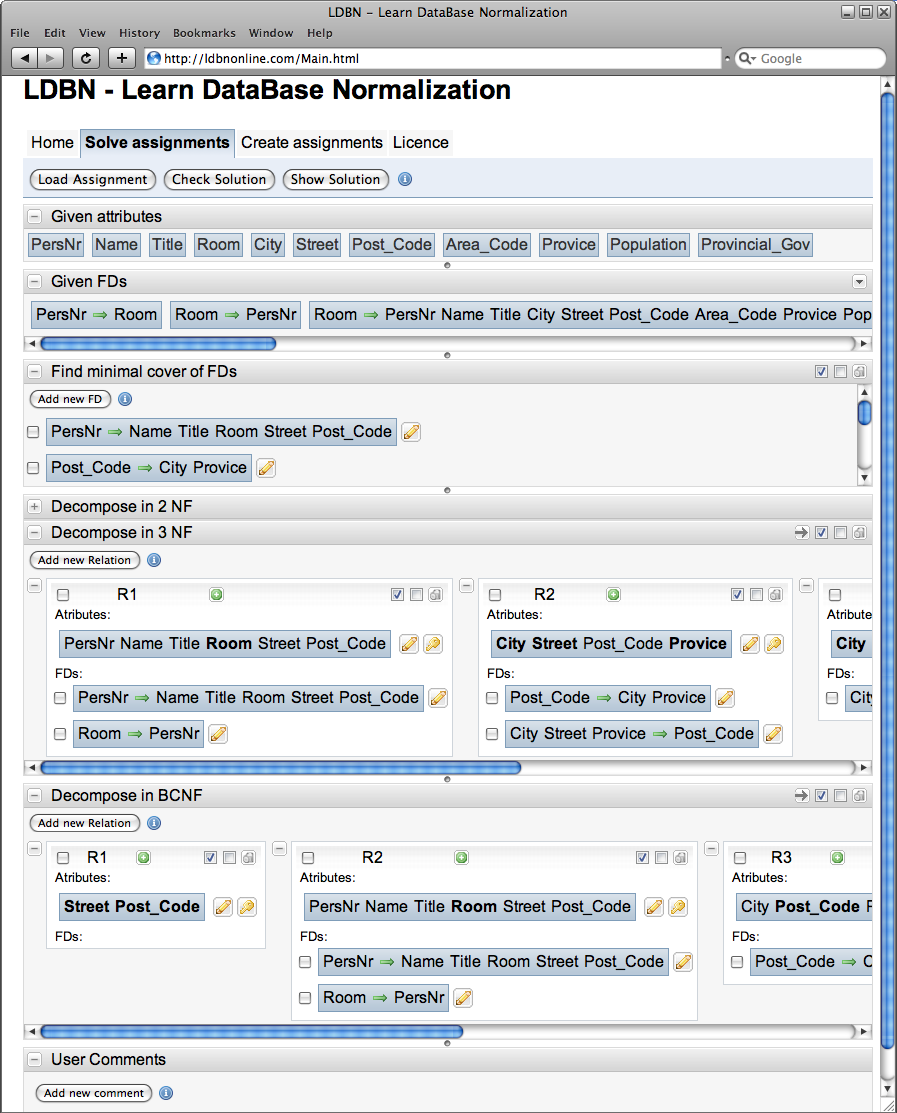
\includegraphics[width=0.8\textwidth]{./img/screen01b.png}
		\caption{LDBN - Solve Assignments Tab}
		\label{fig:screen01}
	\end{center}
\end{figure}

\begin{figure}[h]
	\begin{center}
		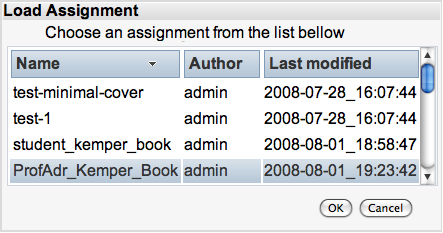
\includegraphics[width=0.6\textwidth]{./img/screen02.png}
		\caption{LDBN - Load Assignments List}
		\label{fig:screen02}
	\end{center}
\end{figure}

The task of checking a potential solution
involves many subtasks which may be performed in any order. In addition to this,  a partial or complete 
solution can be submitted at any given time by pressing the \textit{Check Solution} button. 
After that the system analyzes the solution by performing the following checks:
\begin{enumerate}
	\item Correctness of the minimal cover of the given FDs. 
	\item Losses join properly for every decomposition.
	\item Dependency preservation for every decomposition.
	\item Correctness of the associated with each relation FDs; that is, if the FDs are actually in the embedded closure of F for this relation.
	\item Correctness of the key of each relation.
	\item Correctness of the decomposition, i.e., if the decomposition is really in 2NF, 3NF and BCNF.
\end{enumerate}

\begin{figure}[h]
	\begin{center}
		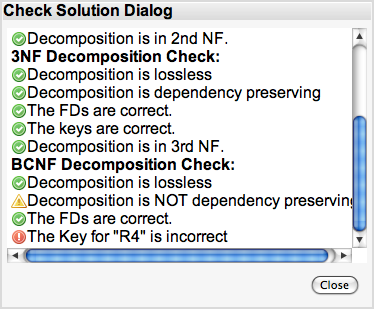
\includegraphics[width=0.6\textwidth]{./img/screen03.png}
		\caption{LDBN - Check Solution Dialog}
		\label{fig:screen03}
	\end{center}
\end{figure}

A dialog with the result is shown to the user. In case of an error the system offers
feedback in form of small textual hints, indicating
where the error might be. Such dialog is shown in Figure~\ref{fig:screen03}. In this case
we can see that the user has made a correct decomposition for 2NF and 3NF,
but his/her decomposition for BCNF has some errors, namely the key of the relation R4 is
incorrect. The dialog is also showing that the decomposition does not 
satisfy the lossless join property, but in the case of BCNF this
is not allays possible, therefore it is only a warning. 

Additional features of LDBN include creating an assignment, which can be done 
only by registered users. This restriction is necessary in order users to be able 
to distinct assignments provided by trusted users, e.g. their database course
lecturers. Registered users have also the ability to leave textual comments 
for every assignment. On the one hand, such
comments ensure that user can easily communicate and share ideas
with each other, and one the other hand, comments could also decrease the amount of workload
for the lecturers in terms of giving an explanation to difficult decomposition.

More detailed and formal description of the features of LDBN will be given in
Chapter~\ref{chap:impl}. 

\section{Comparation of LDBN with Other Tools}
\label{sec:comparation}
In this section we are going to compare LDBN with a couple of other 
available web-based database normalization tools 
such as the \textit{Web-based Tool to Enhance Teaching/Learning Database 
Normalization} by Kung~\cite{p8} and the \textit{The Database Normalization Tool}
\cite{w1}. Furthermore, we are going to discuss why we think our tool is better 
and more efficient
in terms of teaching potential, and give possible reasons why the 
other tools are not commonly used by students.

First of all, the concept of assignments is a major
difference between LDBN and the other normalization tools, 
which only provide 
one possible solution (decomposition) to the user, without users having the ability to test 
themselves. On the other hand, LDBN can be used for checking the correctness of any
arbitrary decomposition, this could be useful for lectures to test handwritten assignments. 

Another major advantage of LDBN over the other tools is the user interface (UI). 
As Frye~\cite{p10} and Dantin~\cite{p9} stated, this is often a
neglected feature, when it comes to educational software. The lack of user-friendly UI 
can often lead to unpopularity of the software among students. An example here could be 
\textit{The Database Normalization Tool}~\cite{w1}. Inputing a relational schema in the program can
take quite sometime due to the fact that
users have to input every attribute manually using the keyboard and then also 
have to input every FD the same way. This may take several minutes even for small  
assignments. Furthermore, relational schemas cannot be saved for future use like 
in LDBN, and users have to input them again next time. To overcome this slow input of user data, 
LDBN supports Drag and Drop. A feature widely used in desktop
applications, but relatively new to AJAX application such as LDBN. Every attribute
and every FD in LDBN can be dragged and dropped, in order 
to define or modify FDs, key attributes, etc... This ensures a really fast and easy
usage of the tool without the need of a keyboard. It should be mentioned
that inputing attributes the traditional way by typing them is also supported.

Community features like posting comments are not present in the other two web-based 
normalization tools, but we believe they are very important when it comes to educational
software. 

\section{Glossary}
\begin{description}
	\item[2NF, 3NF, BCNF] Second Normal Form, Third Normal Form, Boyce-Codd Normal Form. See Section~\ref{sec:nfintro} for more details.
	\item[AJAX] Asynchronous JavaScript And XML is a group of interrelated web development techniques used for creating interactive web applications, for more details see Section~\ref{sec:ajax}.
	\item[CSS] Cascading Style Sheets is a stylesheet language used to describe the presentation of a document written in HTML.
	\item[DBMS] A database management system (DBMS) is a complex set of software programs that controls the organization, storage, management, and retrieval of data in a database.
	\item[GWT] Google Web Toolkit (GWT) is an open source Java software development framework that allows web developers to create AJAX applications in Java. More details in Section~\ref{sec:gwt}.
	\item[ODBC] Open Database Connectivity (ODBC) provides a standard software API method for using database management systems.
	\item[RPC] Remote procedure call (RPC) is an Inter-process communication technology that allows a computer program to cause a subroutine or procedure to execute in another address space.
	\item[SQL] Structured Query Language, is a computer language designed for the retrieval and management of data in relational database management systems, database schema creation and modification, and database object access control management.
	\item[XMLHttpRequest] is an API that can be used by JavaScript and other web browser scripting languages to transfer asynchronously XML and other text data between a web server and a browser.
\end{description}

\chapter{Preliminaries}
\label{chap:preliminaries}
In this chapter we give a brief introduction to relational-database
normalization. The chapter is intended to be used only as quick reference,
since discussing the relational data model and the relational-database normalization
in detail is beyond the scope of this report. For readers who would like to read
more on the subject we recommend the textbook by Elmasri and Navathe~\cite{bdb1} or
the textbook by Kemper and Eickler~\cite{bdb2} for German-speaking readers, both of which have 
proven to be helpful guides throughout the development process of LDBN. There also
many free on-line resources such as the article 
\textit{A Simple Guide to Five Normal Forms in Relational Database Theory}
by Kent~\cite{p7}.  

\section{Definitions}
In the following we give some very important definitions to some key
concepts in the relational-database
normalization, such as relation, key, functional dependency, lossless-join, 
2NF, 3NF, BCNF and others. We also provide the reader with examples to illustrate the 
different normalization concepts in practice. We follow the notations 
of Kemper and Eickler~\cite{bdb2}.
All of the following definitions excluding the examples are also taken from~\cite[Chapter 6]{bdb2}.  

\subsection{Relation}
In relational databases data are represented in tables/relations. 
The columns in the table/relation identify the attributes, for instance
in a table for storing personal data of students such attributes could be
name, date of birth and so forth. A row or a tuple contains all the data of a single 
instance of the table such as a student named John Doe.
In the relational model, every row must have a unique identification or 
key based on the data. Figure~\ref{fig:rmodel} shows an example of a relation, in which 
the Attribute \textit{Matriculation Number} is the key that uniquely identifies each row/tuple in the relation.

\begin{figure}[h]
  \begin{center}
    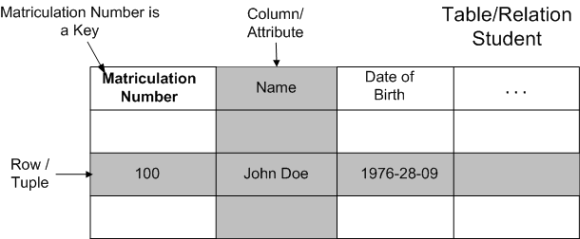
\includegraphics[width=0.85\textwidth]{./img/rmodel01.png}
    \caption{Relation Example}
    \label{fig:rmodel}
  \end{center}
\end{figure}

We would like to give some more formal definitions as well:
\begin{description}
  \item[Relation Schema:] A relation schema is given by a name $R$, together with a finite set
    $Attr(R)$ of attributes. For convenience, when no confusion can result, $R$ will be used as an
    abbreviation for $Attr(R)$.
  \item[Domain:] With each attribute $A \in Attr(R)$ is associated a domain $Dom(A)$, that is
    the set of allowed values for each attribute. 
  \item[Tuple:] A tuple over $R$ is a function $t$ on $Attr(R)$ such that $t(A) \in Dom(A)$
    for each $A \in Attr(A)$. For $\mathbf{B} \subseteq Attr(A)$, the projection of the tuple $t$
    onto $\mathbf{B}$ is is the function $t$ restricted to $\mathbf{B}$.  This
    projection often denoted $t.\mathbf{B}$.  For $\mathbf{B}$ a singleton;
    i.e., $\mathbf{B}=\{C\}$, $t.C$ denotes $t.\{C\}$.
  \item[Relation Instance:] A relation instance $r$ for a relation schema is a set
    of tuples over its attribute set.
  \item[Projection:] Projection is a unary operation written as $\Pi_{\mathbf{B}} (r)$ 
    where $\mathbf{B} \subseteq Attr(A)$  and $r$ is an instance of $R$. 
    $\Pi_{\mathbf{B}} (r) = \{t.\mathbf{B} | t \in r\}$. In words, it deletes attributes that are not in $\mathbf{B}$. 
    Projection operator has to eliminate duplicates.
  \item[Natural Join:] Natural join is a binary operator that is written as $(r \Join s)$ where $r$ and $s$ are relation instances. 
    The result of the natural join is the set of all combinations of tuples in $r$ and $s$ that are equal on their common attribute names.
\end{description}

Subsets of $Attr(A)$ are often written using concatenation, when no
confusion can result.  Thus, if $Attr(A) = \{A,B,C,D\}$, then $\{A,B,C\}$ may
also be written $ABC$. In the following we often use lower-case Greek letters such as
$\alpha$, $\beta$ and $\gamma$ to refer to subset of $Attr(A)$.

\subsection{Key}
As we mentioned a key is used to uniquely identify a tuple. Each table can contain
more than one key. For example,
in our \textit{Student Relation} we could also have an attribute \textit{Personal Number} 
which could also be used
as a key. Furthermore, each key may be composed from more than one attribute, for instance, 
all the attributes of every relation always build a key. However, such a key can often be reduced
to a smaller subset of the relation's attributes. 
We refer to keys that cannot be reduces any more without losing their key property as candidate keys.
In addition, each relation has a primary key, which is a selected candidate key for that relation.

\subsection{Functional Dependency}
The concept of Functional Dependency (FD) is central to normalization theory. 
FD is a semantic concept which describes particular semantic relationship 
between the attributes of a relation. An FD is often represented as $\alpha$ $\rightarrow$ $\beta$, 
where $\alpha$ and $\beta$ are subsets of the attributes of a given relation \textit{R}.
We often refer to $\alpha$ as the left-hand side (LHS) of the FD and to $\beta$ as the 
right-hand side (RHS) of the FD.
The representation $\alpha$ $\rightarrow$ $\beta$ means that for $\beta$ is 
functionally dependent on $\alpha$ if and only if 
for each value of $\alpha$ no more than one value of $\beta$ is associated. 
More formally, if $t$ and $r$ are two tuples in the relation \textit{R}
with $t.\alpha = r.\alpha$ then $t.\beta = r.\beta$. Here
$t.\alpha = r.\alpha$ is a short form for 
\begin{math} \forall A \in \alpha : t.A = r.A \end{math}.  
In other words, the values of the attributes  in $\alpha$ uniquely 
determines the values of of the attributes in $\beta$ and 
if there were several tuples that had the same value of $\alpha$ then all these 
tuples will have an identical values for the attributes in $\beta$. 

We would like to illustrate this very important concept of FDs with an example. 
Let us consider the following relation $R = \{A, B, C, D\}$. 
The example comes from~\cite[Section 6.1]{bdb2}.

\begin{center}
\begin{tabular}[h]{l|l|l|l|l|}
  \cline{2-5}
  & \multicolumn{4}{|c|}{$R$} \\ \cline{2-5}
  & $A$ & $B$ & $C$ & $D$ \\ \cline{2-5}
  $t$ & $a_4$ & $b_2$ & $c_4$ & $d_3$ \\ 
  $p$ & $a_1$ & $b_1$ & $c_1$ & $d_1$ \\ 
  $q$ & $a_1$ & $b_1$ & $c_1$ & $d_2$ \\ 
  $r$ & $a_2$ & $b_2$ & $c_3$ & $d_2$ \\ 
  $s$ & $a_3$ & $b_2$ & $c_4$ & $d_3$ \\ \cline{2-5}
\end{tabular}
\end{center}

It this instance $A \rightarrow B$  is satisfied.
As all $A$ tuples that have the same value have the same $B$ value. However,
$B \rightarrow A$ is \textbf{not} satisfied, since the tuples $r$ and $s$ with $r.B = s.B$ have
different $A$ values. Other FDs on the relation which are also satisfied are
$A \rightarrow C$ and $CD \rightarrow B$.

Functional dependency is \textit{trivial} if it satisfied by all tuples, i.e., $\alpha$ $\rightarrow$ $\alpha$.
In general, a functional dependency of the form $\alpha$ $\rightarrow$ $\beta$ is trivial if 
$\beta \subseteq \alpha$.

\subsection{Closure of a Set of FDs}
In a relation schema $R$ constrained by a set of FDs $F$ we define the closure of $F$ or simply $F\sp{+}$
as a set of all possible FDs which can be derived from the original set of FDs $F$. In 
other words, $F\sp{+}$ is the set of all FDs that must always hold in $R$. $F\sp{+}$ can be
computed using inference rules called \textit{Armstrong's Axioms}. 
Repeated application of these rules will generate all functional dependencies in the closure $F\sp{+}$.

Let $\alpha, \beta, \gamma$ and $\delta$ are subsets of the Attributes in $R$, then:

\begin{description}
  \item[Reflexivity Rule] If $\beta \subseteq \alpha$ then $\alpha \rightarrow \beta$.
  \item[Augmentation Rule] If $\alpha \rightarrow \beta$ then $\alpha\gamma \rightarrow \beta\gamma$, where $\alpha\gamma$ is a short form of $\alpha \cup \gamma$.
  \item[Transitivity Rule] If $\alpha \rightarrow \beta$ and $\beta \rightarrow \gamma$ then $\alpha \rightarrow \gamma$.
\end{description}

\noindent Additional rules which can be derived from above axioms:

\begin{description}
  \item[Union Rule] If $\alpha \rightarrow \beta$ and $\alpha \rightarrow \gamma$ then $\alpha \rightarrow \beta\gamma$.
  \item[Decomposition Rule] If $\alpha \rightarrow \beta\gamma$ then $\alpha \rightarrow \beta$ and $\alpha \rightarrow \gamma$.
  \item[Pseudo Transitivity Rule] If $\alpha \rightarrow \beta$ and $\gamma\beta \rightarrow \delta$ then $\alpha\gamma \rightarrow \delta$.
\end{description}

Here follows a short example on how to apply the different rules. 
Let us consider the following relation:\\ \\
\indent $R = \{A, B, C, G, H, I\}$ \\
\indent $F = \{A \rightarrow B, A \rightarrow C, B \rightarrow H, CG \rightarrow H, CG \rightarrow I\} $ \\

Among others the following FDs can be inferred:\\
\indent \begin{tabular}[h]{r l}
  $A \rightarrow H$ & by applying the Transitivity Rule: $A \rightarrow B, B \rightarrow H$ \\
  $CG \rightarrow HI$ & by  applying the Union Rule: $CG \rightarrow H, CG \rightarrow I$ \\
  $AG \rightarrow I$ & by first applying the Augmentation Rule: $A \rightarrow C, AG \rightarrow CG$; \\
  $ $ & and then applying the Transitivity Rule: $AG \rightarrow CG, CG \rightarrow I$
\end{tabular}

\subsection{Formal Definition of Keys}
With the help of FDs we can now define keys of a relation more formally. 
But first we define 
the concept of \textbf{full functional dependence}. 
Let $\alpha$ and $\beta$ be sets of attributes.
$\beta$ is \textbf{fully functionally dependent} on $\alpha$ if both of the following criteria are true:
\begin{enumerate}
  \item $\alpha \rightarrow \beta$ holds
  \item $\alpha$ cannot be reduced, i.e., $\forall A \in \alpha : \alpha - \{A\} \nrightarrow \beta$ 
\end{enumerate}
 
Let $R$ be a relation with $\alpha \subseteq R$, then $\alpha$ is a \textbf{superkey} if $\alpha \rightarrow R$. 
$\alpha$ is called \textbf{candidate key} if $R$ is fully functional dependent on $\alpha$. 
There can be many candidate keys in a relation. Each relation has one \textbf{primary key},
which is a selected candidate key. Furthermore, we define an attribute as \textbf{prime} or
\textbf{key attribute} if 
it is part of some candidate key of $R$. 

\subsection{Cover of Sets of FDs}
Equivalent sets of functional dependencies are called covers of each other.
There are many different equivalent sets of FDs. 

Two sets of FDs $F$ and $G$ are equivalent ($F \equiv G$)
if and only if their closures are equal, i.e., $F\sp{+} = G\sp{+}$. 
This means for a given set of FDs $F$ there is 
only one unique closure $F\sp{+}$~\cite[Section 6.3.1]{bdb2}. Furthermore every set of functional dependencies 
has a minimal cover~$F_c$. Unlike the closure~$F\sp{+}$ the minimal cover~$F_c$ is not unique. 
A subset $F_c \subseteq F$ is a minimal cover if the following three
properties are satisfied:

\begin{enumerate}
  \item $F_c \equiv F$, i.e., $F\sb{c}\sp{+} = F\sp{+}$
  \item We cannot delete any attribute from any FD and have an equivalent set of FDs.
  \item Every left-hand side of each FD must be unique, thus
    rules with identical LHSs may be combined by combining their RHS.
    This can be done by successively applying the \textit{Union Rule}.
\end{enumerate}

An example: for the relational scheme $R = \{A, B, C\}$, and the set $F$ of functional dependencies: \\

$ F = \{A \rightarrow BC, B \rightarrow C, A \rightarrow B, AB \rightarrow C\}$ \\
\indent The set $F_c = \{A \rightarrow B, B \rightarrow C\}$ is a minimal cover of $F$. \\
\indent Proof:
\indent \begin{enumerate}
  \item $F \equiv F_c $, by applying the \textit{Armstrong's Axioms} it can be shown that $A \rightarrow BC$ and $AB \rightarrow C$ are in $F\sb{c}\sp{+}$, thus the two sets are equivalent.
  \item We cannot remove any attributes from the two FDs in $F_c$, because by doing so they will become trivial and the resulted set will not be equivalent to $F_c$.
  \item The FDs in $F_c$ differ in their LHSs. 
\end{enumerate}

\subsection{Decomposition of Relations}
\label{sec:decofrel}
Relational-database normalization typically involves decomposing a relation $R$
into two or more relations $R_1,...,R_n$, with $R_i \subseteq R$ for each $i$, i.e., the 
new relations contain a subset of the original attributes. 
In order for a decomposition to yield
exactly the same information as the original relation the new relations have to be
combined (joined). However, there are two major criteria that have to be considered when
decomposing a relation:

\begin{enumerate}
  \item \textit{Lossless-Join Property:} ensures that no information is lost during the decomposition process.
  \item \textit{Dependency Preservation Property:} ensures that all the FDs from the original relation hold in the new set of relations. 
\end{enumerate}

\subsubsection{Lossless-Join Property}
The decomposition of $R$ into $R_1,...,R_n$ has a \textit{lossless-join} if for
any instance $r$ of $R$ that satisfies the condition: 
\[
r = r_1 \Join ... \Join r_n \mbox{, with } r_i \mbox{ is the short form of } \Pi_{R_{i}} (r) \mbox{ for } 1 \leq i \leq n
\] 
Thus the information contained in $r$ must be reconstructible by using the natural join~($\Join$) on the relations $R_1,...,R_n$. 

We can also define criteria for the lossless-join property by using FDs. 
A decomposition of $R$ into $R_1$ and $R_2$ has lossless-join
if at least one of the following FDs are in $F\sp{+}$:
\begin{enumerate}
  \item $R_1 \cap R_2 \rightarrow R_1 $ 
  \item $R_1 \cap R_2 \rightarrow R_2 $
\end{enumerate}

The above conditions ensure that the attributes involved in the natural join 
($R_1 \cap R_2$) build a candidate key for at least one of the two relations. This ensures that 
we can never get the situation where spurious tuples are generated, as for any 
value on the join attributes there will be a unique tuple in one of the relations. 

Figure~\ref{fig:lossy} is illustrating a decomposition of a relation $R = \{A, B, C \}$ with
a set of FDs $F = \{B \rightarrow C, C \rightarrow B\}$. As can be seen, the decomposition does
not satisfy the lossless-join property. We can also prove this by showing that the FDs: 
$A \rightarrow AC \notin F\sp{+}$ and $A \rightarrow AB \notin F\sp{+}$.
Figure~\ref{fig:lossless} shows
a lossless-join decomposition of the same relation. Here the requirement for the 
lossless-join property is satisfied,
since $C \rightarrow BC \in F\sp{+}$.

\begin{figure}[h]
  \centering
  \subfigure[Lossy]{
    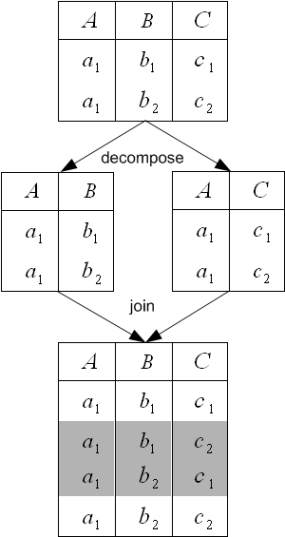
\includegraphics[scale=0.5]{./img/lossy01.png}
    \label{fig:lossy}
  }
  \subfigure[Lossless]{
    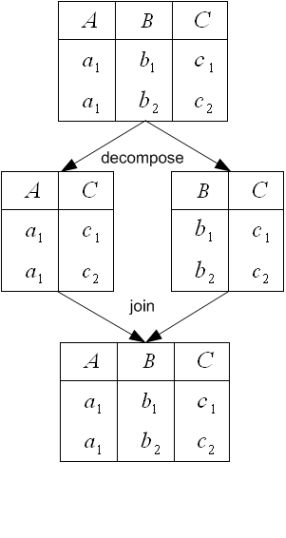
\includegraphics[scale=0.5]{./img/lossless01.png}
    \label{fig:lossless}
  }
\caption{Lossless-Join Property Example}
\end{figure}

\subsubsection{Dependency-Preservation Property}
Another desirable property in database design is dependency preservation. 
Let $F$ be a set of FDs that hold in $R$, which is decomposed in relations $R_1 ,..., R_n$.
Let $F_i$ denote the subset of $F$ consisting of those FDs whose LHS
and RHS both are contained in $R_i$. Then the decomposition is
dependency preserving if the following condition is satisfied: 
\begin{displaymath}
F \equiv (F_1 \cup ... \cup F_n ) \mbox{  respectively  } F\sp{+} = (F_1 \cup ... \cup F_n )\sp{+}
\end{displaymath}

In the following we illustrate the concept of dependency preservation with an example
of a decomposition which is does not satisfy this property: \\ \\
\indent $R = \{A, B, C, D\}$ \\
\indent $F = \{ABC \rightarrow D, D \rightarrow AB\}$ \\
\indent Decompose $R$ in: \\
\indent \begin{tabular}[h]{l l}
  $R_1 = \{C, D\}$  & $F_1 = \{ \}$ \\
  $R_2 = \{A,B,D\}$ & $F_2 = \{D \rightarrow AB \}$ \\
\end{tabular} \\

The decomposition is lossless-join, since $D \rightarrow ABD \in F\sp{+}$. However, 
the decomposition is \textbf{not} dependency preserving, because the FD $ABC \rightarrow D \in F\sp{+}$ but it is
not present in $(F_1 \cup F_2)\sp{+}$.

\section{Brief Introduction to the Normal Forms}
\label{sec:nfintro}
In the previous section we discussed some aspects on how to decompose a relation correctly, 
in this section we will continue this discussion by introducing some of the normal forms
namely the Fist Normal Form (1NF), Second Normal Form (2NF), Third Normal Form (3NF) and
Boyce-Codd Normal Form (BCNF). Normal forms are formal
notations, which are used to avoid or eliminate the three types of data anomalies 
(insertion, deletion and update anomalies) which a database may suffer from. 
These concepts are clarified in the next section, after that we
define the different normal forms.

\subsection{Data Anomalies}
A relation that is not sufficiently normalized can suffer from logical inconsistencies of various types
called data anomalies. We illustrate the the different data anomalies by
giving an example of a relation which suffers from all three anomalies: Insertion, Update and
Delete Anomaly. Table~\ref{fig:relsc1nf}
shows the relation \textit{Student Courses}, which stores data about a student and the courses 
that he/she has taken. In addition, each student is assigned a mentor, who is 
a professor from the student's department. 

%\bgroup
%\setlength\LTleft{-2cm}\setlength\LTright{-2cm}%
%\LTXtable{\textwidth}{./tex/relation-sc.tex}
%\egroup

%\begin{sidewaystable}
%\begin{figure}[h]
%  \begin{center}
%    \begin{longtable}{|C|c|c|c|c|c|c|c|c|C|}
  \hline
  \multicolumn{10}{|c|}{\textit{Student Courses}} \\ \hline 
  \textbf{Matrl.} & Surname & Date of    & Mentor & Mentor  & Mentor   & \textbf{Course} & Course    & ECTS    & Grade \\* 
  \textbf{Nr.}    &         & Birth      & ID     & Surname & Office   & \textbf{Code}   & Name      & Credits &       \\ 
  \hline \hline
  100 & John     & 1976-09-28 & 101 & Codd   & B707 & 5DV001 & Database    & 7.5 & A \\ 
      &          &            &     &        &      &        & Concepts    &     &   \\ \hline
  100 & John     & 1976-09-28 & 101 & Codd   & B707 & 5DV002 & Operating   & 7.5 & B \\
      &          &            &     &        &      &        & Systems     &     &   \\ \hline
  200 & Schmidt  & 1986-05-19 & 201 & Turing & A612 & 5DV001 & Database    & 7.5 & B \\
      &          &            &     &        &      &        & Concepts    &     &   \\ \hline
  200 & Schmidt  & 1986-05-19 & 201 & Turing & A612 & 5DV002 & Operating   & 7.5 & B \\
      &          &            &     &        &      &        & Systems     &     &   \\ \hline
  200 & Schmidt  & 1986-05-19 & 201 & Turing & A612 & 5DV003 & Computer    & 7.5 & C \\
      &          &            &     &        &      &        & Networks    &     &   \\ \hline
  300 & Eriksson & 1984-02-29 & 101 & Codd   & B707 & 5DV004 & Distributed & 7.5 & A \\ 
      &          &            &     &        &      &        & Systems     &     &   \\ \hline
\end{longtable}
%    \caption{Relation \textit{Student Courses}}
%    \label{fig:relsc1nf}
%  \end{center}
%\end{figure}
%\end{sidewaystable}

\begin{sidewaystable}
\begin{center}
\begin{longtable}{|C|c|c|c|c|c|c|c|c|C|}
  \hline
  \multicolumn{10}{|c|}{\textit{Student Courses}} \\ \hline 
  \textbf{Matrl.} & Surname & Date of    & Mentor & Mentor  & Mentor   & \textbf{Course} & Course    & ECTS    & Grade \\* 
  \textbf{Nr.}    &         & Birth      & ID     & Surname & Office   & \textbf{Code}   & Name      & Credits &       \\ 
  \hline \hline
  100 & John     & 1976-09-28 & 101 & Codd   & B707 & 5DV001 & Database    & 7.5 & A \\ 
      &          &            &     &        &      &        & Concepts    &     &   \\ \hline
  100 & John     & 1976-09-28 & 101 & Codd   & B707 & 5DV002 & Operating   & 7.5 & B \\
      &          &            &     &        &      &        & Systems     &     &   \\ \hline
  200 & Schmidt  & 1986-05-19 & 201 & Turing & A612 & 5DV001 & Database    & 7.5 & B \\
      &          &            &     &        &      &        & Concepts    &     &   \\ \hline
  200 & Schmidt  & 1986-05-19 & 201 & Turing & A612 & 5DV002 & Operating   & 7.5 & B \\
      &          &            &     &        &      &        & Systems     &     &   \\ \hline
  200 & Schmidt  & 1986-05-19 & 201 & Turing & A612 & 5DV003 & Computer    & 7.5 & C \\
      &          &            &     &        &      &        & Networks    &     &   \\ \hline
  300 & Eriksson & 1984-02-29 & 101 & Codd   & B707 & 5DV004 & Distributed & 7.5 & A \\ 
      &          &            &     &        &      &        & Systems     &     &   \\ \hline
\end{longtable}
\caption{Relation \textit{Student Courses}}\label{fig:relsc1nf}
\end{center}
\end{sidewaystable}

\begin{description}
  \item[Insertion Anomaly] means that that some data can not be 
    inserted in the database. For example we can not add a new course to the \textit{Student Courses}
    relation, unless we insert a student who has taken that course.
  \item[Update Anomaly] means we have data redundancy in the database and to make any 
    modification we have to change all copies of the redundant data or else the 
    database will contain incorrect data. For example in our database we have the course 
    \textit{Database Concepts} which appears in several tuples in our relation. 
    To change its description to \textit{New Database Concepts} we have to change 
    it in all tuples. Indeed one of the purposes of normalization is to eliminate data 
    redundancy in the database.
  \item[Deletion Anomaly] means deleting some data cause other information to be lost. 
    For example if student Eriksson is deleted from the relation we also lose the 
    information that we had a course \textit{Distributed Systems}.
\end{description}

\subsection{First Normal Form} 
A relation is in first normal form (1NF) if each of
the domains of its attributes is simple or atomic. 
In other words, none of the attributes of the relation is a compositition of multiple attributes, 
a set of values nor a relation. The following relation is not in 1NF:

\begin{center}
\begin{tabular}[h]{|l|l|l|l|}
  \hline
  Matrl.Nr. & Surname & Date\_of\_Birth & Taken\_Courses \\ \hline
  100 & John & 1976-09-28 & \{Database Concepts, Operating Systems \} \\  
  200 & Schmidt & 1986-05-19 & \{Database Concepts, Operating Systems,  \\ 
      &         &            & Computer Networks \} \\
  300 & Eriksson & 1984-02-29 & \{Distributed Systems \} \\ \hline
\end{tabular}
\end{center}

The attribute \textit{Taken\_Courses} is violating the 1NF rule, since it is a set of 
course names. To avoid this we can use a relation similar to the \textit{Student Courses} relation,
which is in 1NF. However, it was shown in the previous section that the relation suffers
from all three data anomalies, therefore we need further restrictions to the 1NF. We
introduce these in the following sections.  

\subsection{Second Normal From}
A relation is in 2NF if it is in 1NF and all its non-key attributes are fully
functionally dependent on every candidate key of the relation.
Note that key attributes are those attributes which are parts of any 
candidate key, and non-key attributes do not participate in any candidate key. 

The relation \textit{Student Courses} is not in 2NF. In order to prove this we must
fist define a set of FDs on the relation. Figure~\ref{fig:fds01a} is a graphical representation 
of the FDs between the primary key \textit{\{Matrl.Nr., Course ID\}} and the rest of the 
attributes in the \textit{Student Courses} relation. 
Note that the attribute to the right of the arrow is functionally dependent on the attribute 
in the left of the arrow.  

\begin{figure}[h]
  \begin{center}
    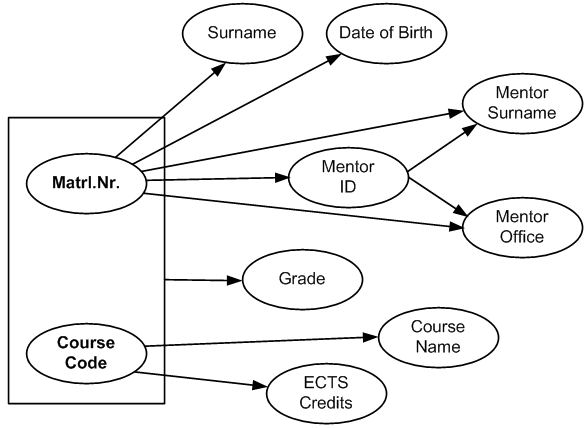
\includegraphics[width=0.6\textwidth]{./img/fds01a.png}
    \caption{Set of FDs which hold in \textit{Student Courses}}
    \label{fig:fds01a}
  \end{center}
\end{figure}

As can be seen only the \textit{Grade} attribute is fully functionally dependent on the primary key.
On the other hand, the attributes \textit{Surname, Date\_of\_Birth, Mentor\_ID, Mentor\_Surname, Mentor\_Office, Course\_Name, ECTS\_Credits} 
and \textit{Grade} are all non-key attributes because non of them is a component of a candidate key, therefore
the relation is not in 2NF. 

To convert \textit{Student Courses} to 2NF we have to make all non-primary attributes 
to be fully functionally dependent on the primary key. 
To do that we need to decompose the \textit{Student Courses} relation into the following three new relations:
\textit{Student and Mentors = \{Matrl.Nr., Surname, Date\_of\_Birth, Mentor\_ID, Mentor\_Office, Mentor\_Surname\}}, 
\textit{Courses = \{Course\_ID, Course\_Name, ECTS\_Credits\}} and 
\textit{Grades = \{Matrl.Nr., Course\_ID,  Grade\}}.
Figure~\ref{alg:relsc2nf} shows these three relations and their contents.


\begin{figure}[h]
\hrule
\vspace{0.25cm}
\begin{center}
\begin{tabular}[h]{|c|c|c|c|c|c|}
\hline
\multicolumn{6}{|c|}{\textit{Students and Mentors}} \\ \hline
\textbf{Matrl.Nr.} & Surname & Date\_of\_  & Mentor\_ & Mentor\_  & Mentor\_ \\
                   &         & Birth       & ID       & Surname   & Office \\
 \hline \hline
 100 & John     & 1976-09-28 & 101 & Codd   & B707 \\
 200 & Schmidt  & 1986-05-19 & 201 & Turing & A612 \\
 300 & Eriksson & 1984-02-29 & 101 & Codd   & B707 \\ \hline
\end{tabular} 
\end{center}

\vspace{0.5cm}

\begin{minipage}[t]{0.5\linewidth}
\centering
\begin{tabular}[h]{|c|c|c|}
\hline
\multicolumn{3}{|c|}{\textit{Courses}} \\ \hline
\textbf{Course\_} & Course\_Name & ECTS\_ \\
\textbf{Code} &  & Credits \\
\hline \hline
5DV001 & Database Concepts   & 7.5 \\ 
5DV002 & Operating  Systems  & 7.5 \\
5DV003 & Computer  Networks  & 7.5 \\
5DV004 & Distributed Systems & 7.5 \\ \hline
\end{tabular}

\end{minipage}
\hspace{0.5cm}
\begin{minipage}[t]{0.5\linewidth}
\centering
\begin{tabular}[h]{|c|c|c|}
  \hline
  \multicolumn{3}{|c|}{\textit{Grades}} \\ \hline
  \textbf{Matrl.Nr.} & \textbf{Course\_} & Grade \\
   & \textbf{Code} &  \\
  \hline \hline
  100 & 1 & A \\ 
  100 & 2 & B \\
  200 & 1 & B \\
  200 & 2 & B \\
  200 & 3 & C \\
  300 & 4 & A \\ \hline
\end{tabular}
\end{minipage}

\caption{Decomposition of Relation \textit{Student Courses} in 2NF}\label{alg:relsc2nf}
\hrule
\end{figure}

All three relations are in 2NF. Furthermore, it can be proven that the
decomposition is lossless-join and dependency preserving. 
Examination of the new relations shows that we have eliminated most of the redundancy 
in the database. The relations \textit{Courses} and \textit{Grades} are free
from any data anomalies. However, the \textit{Students~and Mentors} relation still suffers form all three
data anomalies, because it also keeps track of all mentors:
\begin{enumerate}
  \item We cannot add new mentors without adding new students.
  \item To change the office of a mentor we have to update several tuples.
  \item If the student Schmidt is deleted we also lose the information about the mentor Turing.
\end{enumerate}
 
\subsection{Third Normal Form}
A relation $R$ is in 3NF if it is in 2NF and for all FDs that hold in $R$
of the form $\alpha \rightarrow B$, where $\alpha \subseteq  R$ and $B \in R$, 
at least one of the following holds: 
\begin{enumerate}
  \item $B \in \alpha$, i.e., the FD is trivial
  \item $B$ is a prime attribute, i.e., $B$ is part of a candidate key.
  \item $\alpha$ is a superkey of $R$.
\end{enumerate}

From the three previous relations only \textit{Students and Mentors} is not in 3NF, since 
the FD \textit{Mentor~ID $\rightarrow$ Mentor~Surname, Mentor~Office} holds in the relation but 
it violates the 3NF property. Therefore we need to further decompose the relation into two
new relation: \textit{Students~= \{Matrl.Nr., Surname, Date\_of\_Birth, Mentor\_ID\}} and
\textit{Mentors~= \{Mentor\_ID, Mentor\_Surname, Mentor\_Office\}}.
Figure~\ref{alg:relsc3nf} shows the two new relations and their content.

\begin{figure}[h]
\hrule
\vspace{0.25cm}
\begin{minipage}[t]{0.5\linewidth}\centering
\begin{tabular}{|c|c|c|c|}
\hline
\multicolumn{4}{|c|}{\textit{Students}} \\
\hline
\textbf{Matrl.Nr.} & Surname & Date\_of\_  & Mentor\_ \\
                   &         & Birth    & ID\_     \\
\hline \hline
100 & John     & 1976-09-28 & 101 \\
200 & Schmidt  & 1986-05-19 & 202 \\
300 & Eriksson & 1984-02-29 & 101 \\
\hline
\end{tabular}
\end{minipage}
\hspace{0.5cm}
\begin{minipage}[t]{0.5\linewidth}\centering
\begin{tabular}{|c|c|c|}
\hline
\multicolumn{3}{|c|}{\textit{Mentors}} \\ \hline
 \textbf{Mentor\_} & Mentor\_  & Mentor\_ \\
 \textbf{ID}       & Surname   & Office \\
 \hline \hline
 101 & Codd   & B707 \\
 201 & Turing & A612 \\ \hline
\end{tabular}
\end{minipage}

\caption{Decomposition of Relation \textit{Students and Mentors} in 3NF}\label{alg:relsc3nf}
\hrule
\end{figure}

It can be shown that the two new relations are in 3NF. Furthermore, the 
decomposition has the lossless-join and dependency-preserving properties. Indeed, it is always 
possible to find a dependency-preserving, lossless-join decomposition which is in 3NF~\cite[Section 6.8]{bdb2}.
However, a 3NF decomposition does not necessarily satisfy these properties. Consider the following example
of a 3NF decomposition which is not dependency preserving:

\begin{center}
\begin{tabular}[h]{l l}
  $R = \{A, B, C, D\}$ & $F = \{A \rightarrow BC, C \rightarrow D, D \rightarrow B\}$ \\
  Decompose $R$ in:  & $R_1 = \{A, B, C\} \mbox{ and } R_2 = \{C,D\}$ \\ 
\end{tabular}
\end{center}

Returning to the running example, it is worth noting that our original relation \textit{Student Courses} is now decomposed
into four different relations: \textit{Students, Mentors, Courses} and \textit{Grades}. The 
decomposition is in 3NF, this means that each member of the set of relation schemes is in 3NF. 
More importantly, the decomposition does not suffer any data anomalies. 
Let us clarify this in more detail:
\begin{description}
  \item[Insertion Anomaly:] Now new mentors and courses can be inserted to the relation \textit{Mentors}/\textit{Courses} without needing to add new students.
  \item[Update Anomaly:] Since redundancy of the data was eliminated no update anomaly can occur. For example, to change the \textit{Course Name} for 5DV001 only one change is needed in the relation \textit{Courses}.
  \item[Deletion Anomaly:]  The deletion of student Schmidt from the database is achieved by deleting Schmidt's records from both \textit{Students} and \textit{Grades} relations and this does not have any side effects on the different courses or mentors, since they stay untouched in their own relations.  
\end{description}

\subsection{Boyce-Codd Normal Form}
\label{sec:BCNF}
BCNF is a slightly stronger version of 3NF. A relation scheme $R$ is in BCNF 
with respect to a set $F$ of FDs if $R$ is in 3NF and for all functional dependencies in $F\sp{+}$ 
of the form $\alpha \rightarrow \beta$, where $\alpha \subseteq R$ and $\beta \subseteq R$,
at least one of the following holds:
\begin{enumerate}
  \item $\alpha \rightarrow \beta$ is a trivial functional dependency (i.e. $\beta \subseteq \alpha$)
  \item $\alpha$ is a superkey for $R$ 
\end{enumerate}

Only in rare cases a 3NF relation does not meet the requirements of BCNF. In fact, our decomposition 
\textit{\{Students, Mentors, Courses, Grades\}} is in BCNF. Let us consider the following
example of a relation which is in 3NF but not in BCNF.  The example 
comes from~\cite[Section 6.5.3]{bdb2}.

\begin{center}
\begin{tabular}[h]{l l}
  $PostalCodeIndex = \{Street, City, Province, PostalCode\}$ & \\ [0.5ex]
  $F = \{Street, City, Province \rightarrow PostalCode; \mbox{ } PostalCode \rightarrow City, Province\}$ \\ [1.5ex]
  The FD $PostalCode \rightarrow City, Province$ is not trivial and it is not a superkey, \\ [0.5ex]
  thus the $PostalCodeIndex$ relation is not in BCNF. & \\ [1.5ex]
  BCNF decomposition of $PostalCodeIndex$:   &  \\ [0.5ex]
  $Streets =\{PostalCode, Street\}$ & \\ [0.5ex]
  $Cities = \{PostalCode, City, Province\}$ & \\ [0.5ex]
\end{tabular}
\end{center}

The decomposition \textit{\{Streets, Cities\}} is lossless-join, but it is not dependency-preserving. 
Indeed, some schemata do not have dependency-preserving decompositions
into BCNF, as such they are considered pathological by some.

\chapter{Design Concepts}
\label{chap:design}
In this chapter we discuss some design decisions of LDBN such as
reasons for moving to a web-based application, platform choice and 
design ideas which were considered but not included in the final version. In the following the
term client is used to refer to a browser.

\section{Choice of Platform}
Due to the fact that web-enabled educational 
systems are becoming the dominant type of systems 
available to students, we designed LDBN as a web-based application.
In addition to this, web-based systems offer several advantages in comparison to 
standalone systems. They minimize the problems of distributing software to users 
and hardware and software compatibility. New releases of systems are immediately
available to everyone. More importantly, students are not
constrained to use specific machines in their schools, and can access 
web-based applications from any location and at any time. This type of independence 
is of enormous value for learning environments due to the importance of
flexibility and accessibility for the learning process.
 
The main issue, which really lies within the choice of platform, is the fact that there are
many different techniques for implementing a web-based application. A basic HTML-based
solution would not work since all pages in that case would be static. The remaining 
options can be divided into three groups:

\begin{enumerate}
	\item Client-side based
	\item Server-side based
	\item Client-server based
\end{enumerate}

The client-side solution consists of an application which runs entirely on the user's 
computer within a browser. Examples here could be the Java Applet, the Adobe Flash or the new 
Microsoft Silverlight technologies. However, this approach has the disadvantage
of requiring a plug-in, which is not always available by default on all web browsers. 
In addition, some organizations only allow software installed by the administrators. 
As a result, many users cannot view neither Java applets nor Adobe Flash by default. This could 
have a negative impact on the accessibility of an application; 
therefore we did not proceed with the client-side approach.

In the server-side solution there is a web server and optionally a data service. 
Web servers such as Apache, Tomcat, Lighttpd and IIS host the application 
logic, which is written in Java, PHP, Ruby, C\# or other languages. 
Data services are provided by databases systems such as MySQL, Oracle, SQL Server and 
so forth. This approach has a centralized architecture; thus all tasks and 
functions are performed on the server. After their completion a new HTML page is 
sent back to the client. This approach has two major drawbacks. In the first place, 
the browser must re-render the whole HTML page after each interaction with the server.
Although part of this could be avoided with the help of frames, it would still 
require more data than actually needed to be sent back to the client, since most 
parts of the page remain the same after each interaction. In the second place, 
all of the computations must be done on the server-side, leaving the client with 
the only task of rendering a page. This may result in a poor allocation of computational tasks. 
With the introduction of rich web-applications such as Google Maps, Facebook, 
Google Docs and others it has been shown in practice that the client is capable of 
much more than simply rendering a web page. 

Finally, there are client-server-based solutions, such as those
which use packages such as AJAX, which could be
seen as a mixture 
of the first two solutions. As it is used by LDBN, we
discuss AJAX more formally in the following section.

\section{AJAX}
\label{sec:ajax}
AJAX stands for Asynchronous JavaScript And XML. It should be noted
that AJAX is not a new technology in itself but rather the integration of several 
existing technologies, including HTML, CSS and JavaScript~\cite{w3}. Prior to AJAX browsers 
were treated 
like dumb terminals; thus the browser was unable to remember its state and every 
user interaction caused a HTTP round trip over the network, requiring browsers 
to re-render the whole web page after each request. With AJAX browsers became 
more powerful. Traditional web techniques like HTML and CSS are still used to 
render the page. In spite of that, JavaScript can be used to access 
and manipulate the Document Object Model (DOM) tree, i.e., 
JavaScript is capable of changing only certain parts
of the content of a web page. However, the
real potential of AJAX lies within the client-server communication, an example
of which is illustrated in Figure~\ref{fig:ajax01}. In this example we have an AJAX application
which runs within a browser. JavaScript must be enabled in the browser, otherwise
the application will not start.  
The XMLHttpRequest is an API implemented by the browser,
which can be accessed by the application using JavaScript. This API is 
used to handle communication with the server in an asynchronous fashion using a
simple HTTP connection. It is worth mentioning that other solutions also exist. 
For example, XML is often used to transfer data between the server and the client, 
although XML is not required for data interchange and often other text-based
formats are used as an alternative such as JSON or plain text~\cite{bajax1}. In our example we have 
a web server which is used to establish a connection between the AJAX application and
the DBMS, where we store the data.

\begin{figure}[h]
	\begin{center}
		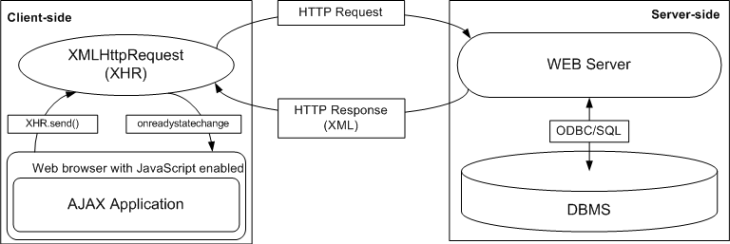
\includegraphics[width=0.8\textwidth]{./img/ajax01a.png}
		\caption{Example of an AJAX Architecture}
		\label{fig:ajax01}
	\end{center}
\end{figure}

Another advantage of AJAX is the so called \textit{Architectural Shift}~\cite{wgdd1}, 
which is illustrated in Figure~\ref{fig:ajax02}, which is
an adaptation of~\cite[Figure 3]{wgdd1}. 
It describes the ability of the client to handle events
locally, without the need of a server. Such events can be for example the
expansion of a tree. This has two advantages. On the one hand, it frees server 
and network resources for other tasks, on the other hand, it allows
the UI to be more interactive and to respond more quickly to inputs.

\begin{figure}[h]
	\begin{center}
		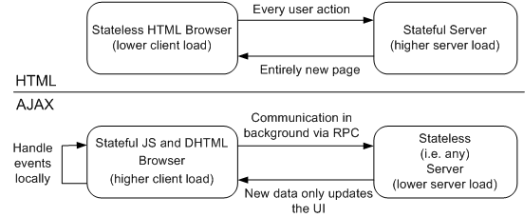
\includegraphics[width=0.8\textwidth]{./img/ajax02a.png}
		\caption{AJAX Architectural Shift}
		\label{fig:ajax02}
	\end{center}
\end{figure}

AJAX has also several shortcomings,
the biggest of which is the fact that it is not a standard. This has led to slight 
differences in the JavaScript language between browsers, along with major differences 
in the DOM and in the XMLHttpRequest API~\cite{bgwt1, bgwt2, bgwt3}. 
For our learning environment we need to support every major browser to ensure accessibility. 
However, this often requires writing a different code base for different browsers,
and this means less scalability for the application and less productivity 
for the developers~\cite{bgwt2}. Another major
disadvantage is the lack of good developer tools for JavaScript~\cite{bgwt2}, which also 
has a negative impact on the scalability and productivity.
A typical example here could be the debugging process of an AJAX project - 
often bugs are caused by a simple typographical error (typo), which in the case 
of JavaScript means that such errors can be found only at run time, and usually 
by end users~\cite{wgdd1}. 
These and other problems related with AJAX
led to the decision to use GWT - Google Web Toolkit~\cite{wgwt}, an introduction 
to which can be found in the following section.

\section{GWT} 
\label{sec:gwt}
Google Web Toolkit (GWT) is a set of tools and libraries that allows
web developers to create AJAX applications in Java~\cite{wgwt}. 
The tools are focused on solving the problem of moving the desktop application into the
browser~\cite{bgwt2}. GWT is an open source project and it is developed 
by Google. The major components of GWT include: 

\begin{enumerate}
	\item Java-to-JavaScript Compiler.
	\item Hosted Web Browser.
	\item JRE emulation library.
	\item Web UI class library.
	\item Many other libraries and APIs.
\end{enumerate}

The most important component is the Java-to-JavaScript compiler. It enables the 
translation of Java code into highly optimized, browser 
independent\footnote{As of GWT version 1.5, GWT supports: 
Firefox 1,~2,~3; Internet Explorer 6,~7; Safari 2,~3; Opera~9}
JavaScript code. 
In addition to this, it provides developers with compile-time error checking. 
Another very important
aspect of the compiler is the fact that when the code is compiled into JavaScript,
it results in 
a single JavaScript file for each browser type and target locale. This is illustrated 
in Figure~\ref{fig:gwt01}, which is an adaptation of~\cite[Figure 7]{wgio2}. 
Typically this means that a GWT application will be compiled into 
a minimum of five separate JavaScript files. Each of these files is meant to run 
on a specific browser type, version, and locale. A bootstrap script, initially 
loaded by the browser, will 
automatically pull the correct file when the
application is loaded. The benefit of this is that the code loaded by the browser 
will not contain code that it cannot use. The JavaScript code produced by the GWT 
compiler is highly optimized and it usually runs much faster than handwritten 
JavaScript code~\cite{wgio1}. Moreover, the development team must support only
one code base, by which the the scalability of an application can be increased.  

\begin{figure}[h]
	\begin{center}
		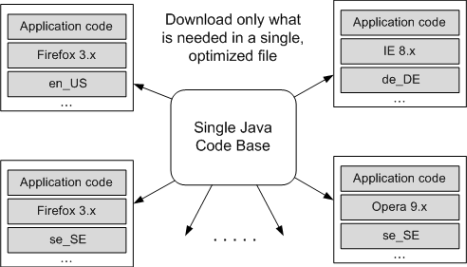
\includegraphics[width=0.8\textwidth]{./img/gwt01a.png}
		\caption{GWT Java-to-JavaScript Compiler}
		\label{fig:gwt01}
	\end{center}
\end{figure}

Another very important component is the hosted web browser. A GWT application can 
be run in hosted mode, this means 
the Java code is not compiled into JavaScript code but rather it is executed natively  
in a special hosted web browser. This browser works like any other web
browser, but it is specifically tailored for GWT development. It allows the developer
to make changes to the Java code and immediately see the results, without the need
of recompiling the source code. Furthermore, the hosted mode allows the use of 
very powerful development tools such as the Java debugger with all its functionality 
including placing a breakpoint. As Bruce Johnson~\cite{wgdd1}, 
the creator of GWT, has stated, before GWT this was nearly an impossible task in 
AJAX applications. With GWT developers can take full advantage of 
already existing development tools such as such as the Eclipse IDE~\cite{weclipse}. 
This can further increase the scalability of an application and the productivity 
of developers. 
In the case of LDBN, GWT helped scale the project to such extent that LDBN runs 
almost entirely on the client-side. In addition, LDBN has grown fast to 
more than 60 classes/interfaces. Debugging such large application without the powerful 
tools provided by GWT and Eclipse would have been nearly an impossible task for 
a single developer.

Other important components of GWT, which were also used in the development 
process of LDBN, include:

\begin{description}
	\item[JRE emulation library] This library contains 
	the most commonly used parts of the full Java Runtime Environment (JRE), 
	which can be compiled into JavaScript. LDBN uses extensively many of the collection 
	classes of the emulated library such as the \verb=ArrayList=, \verb=HashMap=, 
	and others classes.
	\item[Web UI library] GWT includes a large set of UI classes, which 
	enable the development of a web UI entirely in Java. The approach is similar 
	to writing a Java Swing application, and it is used to develop the whole UI 
	of LDBN. 
	\item[DOM API] GWT provides an abstraction on top of the DOM, 
	allowing the use of a single Java API without having to worry about 
	differences in implementations across browsers.
	\item[XML Parser] To make it as simple as possible to deal with XML data formats 
	on the client browser, GWT provides a DOM based XML parser.
	\item[RequestBuilder API] GWT also provides an abstraction on top of the
	XMLHttpRequest object. 
	\item[GWT-RPC] The GWT-RPC mechanism allows Java objects to be sent between 
	the client and the server. However, this is only true for 
	servlet containers such as the Apache Tomcat web server. 
	\item[JSNI] The JavaScript Native Interface (JSNI) makes it possible to
	write native JavaScript code within the Java code. The JavaScript code can 
	then be executed from Java code and vice versa - Java code can be executed
	from JavaScript code. JSNI is very important part of GWT, as it enables 
	the integration with already existing JavaSctipt applications.  
	\item[Internationalization] Several techniques are provided by GWT that can 
	aid with internationalization issues.
	\item[JUnit Integration] GWT provides support for JUnit~\cite{wjunit}, 
	a framework for making automated tests.
\end{description}

For additional literature on the subject of GWT, we recommend the book of 
Ryan Dewsbury \textit{Google Web Toolkit Applications}~\cite{bgwt2}. It has
proven to be very useful information source throughout the development process 
of LDBN.  

\section{Limitations of GWT and JavaScript}
Despite the fact that GWT offers solution to many of the problems
described in Section~\ref{sec:ajax}, it still has to deal with some 
fundamental issues regarding 
AJAX. Although the client-side application is written in Java, 
the code produced by the GWT compiler is still JavaScript, and
as such it has the following limitations:
   
\begin{enumerate}
	\item Single-thread environment.
	\item Same origin policy.
	\item No database connectivity.
\end{enumerate}

There is no way around the single-thread-environment issue. This can cause the UI
to become unusable for a while. In order to provide a more appropriate behavior 
for the UI, LDBN locks the entire UI before every extensive computation; e.g.,
testing the correctness of an assignment. When the UI is locked,
it gets dimmed and an image is indicating that the program is working. After 
completion the UI returns to its normal state. 

The same origin policy prevents AJAX applications from being used across domains,
although the W3C has a draft that would enable this functionality~\cite{bajax1}.

A browser-independent AJAX application is not capable of making a connection 
to a database~\cite{bajax1}, thus it requires a web server to establish the 
connection. Then the client-side communicate with the server-side using 
predefined XML format.

\section{Server-side Platform Choice}
In this section we give our reasons for choosing PHP as the server-side
scripting language and MySQL as the database management system (DBMS). First we would
like to mention that LDBN is open source and it is distributed under the 
Apache License, Version 2.0~\cite{walv2}. Furthermore, we would like to see 
LDBN installed on other servers as well. This could help LDBN become
a leading learning environment across 
different universities for teaching relational-database normalization. To ensure 
portability we have decided to use the most common free 
tools for web development. Apache Web Server with PHP and MySQL meet those requirements. 
Apache is the most popular HTTP server on the Web~\cite{w3} and PHP is the most popular 
Apache module~\cite{w4}. In addition, MySQL is the most popular open source 
database system~\cite{w5}.
 
It is worth mentioning that even though LDBN is implemented using Apache Web Server,
PHP and MySQL, it is possible to use different tools and programming languages 
on the server-side with almost no modifications to the client-side. However, 
the predefined XML data exchange format must stay the same.

\section{Other Design Issues}
An initial design of LDBN included an assignment generator, i.e., assignments were not
created by users, but rather automatically generated. However, this approach
has proven to be highly ineffective in terms of creating good assignments. There 
are many reasons for this, but the main one is the fact that it is not clear how
to determine good assignments. Every assignment could emphasize on different aspects of
the relational-database normalization, thus this approach has been disregarded.


\chapter{Implementation}
\label{chap:impl}
In this chapter we give a formal overview of the system architecture,
some of the core classes and the most important
features of LDBN~- the different normalization algorithms and the user interface. 
In addition, we give an overview
of some key aspects of the server-side implementation and communication
between server and client. At the end of the chapter we go over some
security issues and how LDBN deals with those. 

\section{System Architecture}
Figure~\ref{fig:sysarch} illustrates the architecture of LDBN. 
As can be seen, the architecture is decentralized. The client side implements 
all of the tutoring functions and the server side is used only for storing data.
As it was mentioned earlier, such a decentralized architecture ensures fewer HTTP requests to
the server, which in a single-thread environment as JavaScript means faster 
responses of the UI to user inputs. The architecture also reduces the server load,
which implies that the server can handle more users.

\begin{figure}[h]
	\begin{center}
		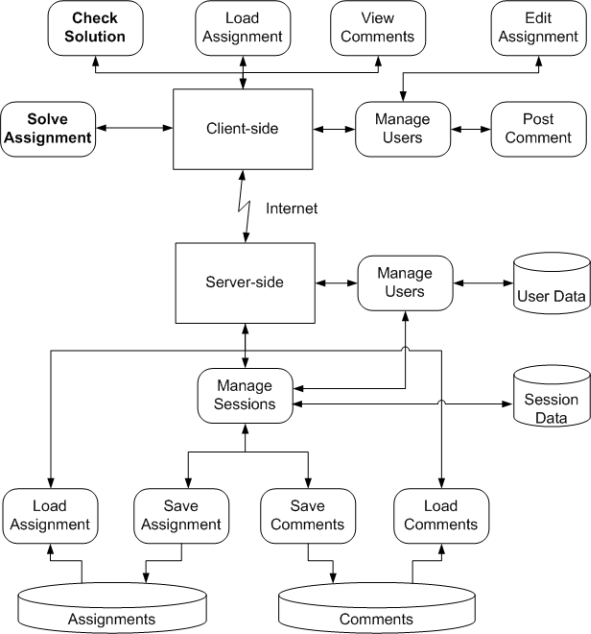
\includegraphics[width=0.85\textwidth]{./img/architecture01a.png}
		\caption{System Architecture of LDBN}
		\label{fig:sysarch}
	\end{center}
\end{figure}

It should be noted that the functions in the diagram represent many classes and 
static methods, which all serve the same purpose/function. We do not 
discuss all 
of the functions in detail, because most of them are straightforward and 
self-explanatory. 

\subsubsection{The Client-Side Functions}

\begin{description}
	\item[The Solve Assignment] function is used for generating a sample solution to 
		a given assignment, and presenting it to the user. As we mentioned in 
		Section~\ref{sec:introldbn}, an assignment consist of a relation schema in universal-relation form (URF).
	\item[The Check Solution] function, as the name suggests, performs series of checks to 
		test the correctness of the given solution. A solution to an assignment consists 
		of a decomposition of the schema from URF into 2NF, 3NF and BCNF. In addition,
		the user must identify one of the candidate keys of each new relation
    in the decomposition as the primary key of that relation.
	\item[The Load Assignment] function presents a list of all assignments, which are 
		stored in the database, to the user, and it can load new assignment from that list
		in the UI.
	\item[The Manage Users] function allows unregistered users to create new accounts 
		and registered users to login with their password and user-name. 
	\item[The Post Comment] function gives registered users the ability to comment an assignment, 
		thus be able to communicate with all other users.
	\item[The View Comments] function displays comments for each assignment, posted by registered users.
	\item[The Edit Assignment] function provides registered users with the 
		ability to create, edit, save, export and import assignments. 
\end{description}

As we can see from Figure~\ref{fig:sysarch} the functions \textit{Post Comments} 
and \textit{Edit Assignments} do not directly communicate with the server side, but rather 
communication goes first trough the \textit{Manage Users} function. This is done in order 
to ensure that the users are properly logged onto the system before attempting 
to use those functions. We will refer to functions which require users to login as restricted. 

The functions \textit{Solve Assignment} and \textit{Check Solution} are definitely the most 
important functions of LDBN, therefore we illustrate how they perform their tasks
in more detail in Section~\ref{sec:keyfunctions}. 

\subsubsection{The Server-Side Functions}
Most of the functions on the server side are used as communication links (CL) for the
functions on the client side to the database. This means they retrieve/store data from/in the 
database, and then convert the data to an XML string and send it back to the client side
functions. 

\begin{description}
	\item[The Load Assignment] function is the CL for the \textit{Load Assignment} function on the 
		client side.
	\item[The Load Comments] function is the CL for the \textit{View Comments} function.
	\item[The Manage Sessions] function ensures that the data are coming from a registered user.
		It is also responsible for creating a new session, and terminating an existing one. Furthermore,
		each session has a unique ID, which is generated and sent back to the user 
		when he/she has logged in. This ID is stored in the \textit{Session Data} and it is used for
		authenticating the user in order for him/her to obtain access to restricted functions.
	\item[The Manage Users] function is the CL of the \textit{Manage Users} on the client side.
		It is responsible 
		for inserting new users into the database and for modifying existing data such as 
		user-name, password and email.
		It uses the \textit{Manage Sessions} function in order to ensure that a
		user is always logged in, before he/she attempts to change any user data.  
	\item[The Save Assignment] function is the CL for the \textit{Edit Assignment} function on the client side. 
		It is a restricted function, thus it uses the \textit{Manage Sessions} function. 
	\item[The Save Comment] function is CL for the \textit{Post Comment} function on the client side, it is 
		a restricted function as well.
\end{description} 

\section{Core Package of LDBN}
\label{sec:corepk}
Before moving to Section~\ref{sec:keyfunctions}, where we discuss the most important functions of 
LDBN namely the \textit{Solve Assignment} and the \textit{Check Solution} functions, 
we present the core package of LDBN. This package contains the foundation 
classes, on which both of the functions depend, therefore it is an essential 
part of LDBN. 

A very important part of LDBN is the representation of sets of attributes, since all 
data items in a database schema are based on sets of attributes. Therefore we developed an
efficient data structure called \verb=AttributeSet=, which holds a (sub)set of attributes of a relation.  
Before going into more detail, we present the different data items in LDBN. 
We refer to data items as items necessary to describe a database schema.  
The three fundamental items in our implementation are relations, FDs, and keys. Furthermore,
we are interested only in candidate keys and primary keys of a relation, not in not in non-minimal superkeys.
Figure~\ref{fig:relexample} illustrates
an (abstract) example of those data items and their structure in our system. 

%\begin{figure}[h]
%  \begin{center}
%    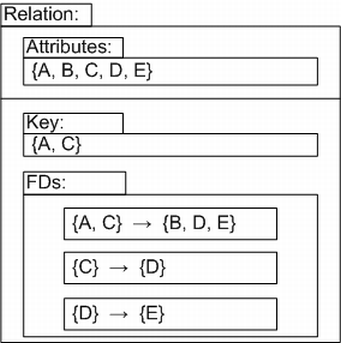
\includegraphics[scale=0.4]{./img/relation-example01a.png}
%    \caption{Example of a Relation}
%    \label{fig:relexample}
%  \end{center}
%\end{figure}

\begin{figure}[h]
  \centering
  \subfigure[Standard Representation]{
    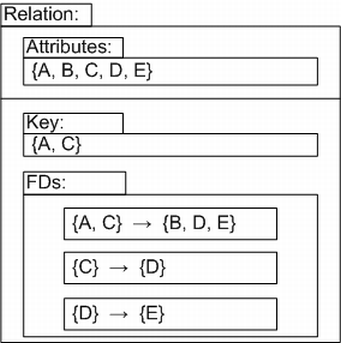
\includegraphics[scale=0.4]{./img/relation-example01a.png}
    \label{fig:relexample}
  }
  \subfigure[Representaion with Respect to AttributeSet]{
    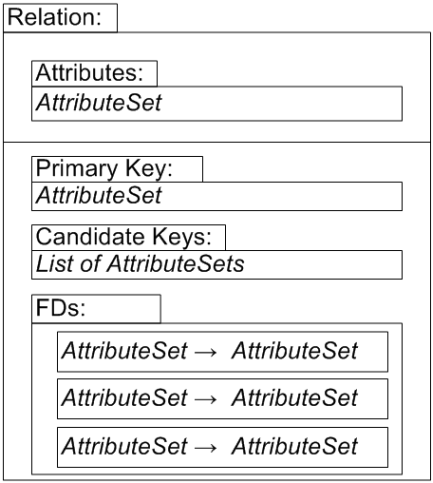
\includegraphics[scale=0.4]{./img/relation-example02a.png}
    \label{fig:relexample2}
  }
\caption{Example of a Relation Representation in LDBN}
\end{figure}

As can be seen, the most important data item is the relation, since
it holds the other two data items. This suggests itself, because FDs and keys have meaningful
interpretation only in combination with a relation. Furthermore, a key is a subset of 
the relation's attributes.
Each relation have a set of candidate keys and one primary key, which is an element form that set. 
Moreover, each relation is assigned a set of FDs. On the other hand, 
each FD consists of two subsets of
the relation's attributes, these represent the left-hand side (LHS) and the 
right-hand side (RHS) of an FD. Finally, a database schema or a decomposition of
a database schema can be described as a set of relations.

As the reader may have noticed, each data item consists of attributes and/or other
data items. Therefore we can use only our data structure \verb=AttributeSet=
in order to describe how the different data items are constructed. 
Figure~\ref{fig:relexample2} shows the same relation as in Figure~\ref{fig:relexample} with
respect to the instances of the \verb=AttributeSet= necessary to construct the different
data items.

%\begin{figure}[h]
%  \begin{center}
%    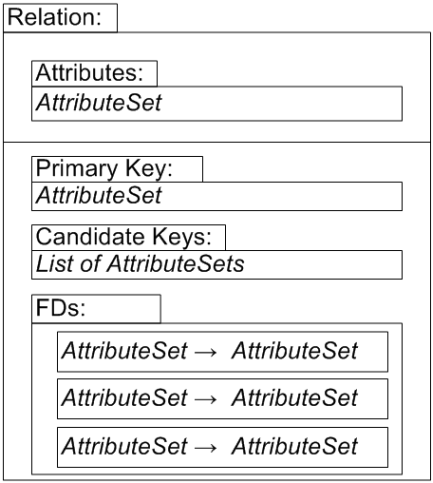
\includegraphics[scale=0.4]{./img/relation-example02a.png}
%    \caption{Example of a Relation with respect to AttributeSet}
%    \label{fig:relexample2}
%  \end{center}
%\end{figure}

As can be seen a (primary) key is simply an instance of \verb=AttributeSet=. The candidate keys
are represented as a list of instances of \verb=AttributeSet=. An FD is constructed from
two instances of \verb=AttributeSet=, one for the LHS and one for the RHS. And finally,
a relation is a composition of an instance of  \verb=AttributeSet= for representing
the relation's attributes, a primary key, a list of candidate keys and a list of FDs. 

Here follows a description of the implementation of the \verb=AttributeSet= data structure. 
In the early stages of the implementation of LDBN the \verb=AttributeSet=
was simply an array of strings. However, this has proven to be very
inefficient even for trivial operations such as comparison or union of two sets. This could 
lead to efficiency problems with
bigger assignments, since set operations are used quite often due to the exponential
complexity of many algorithms in LDBN. 
The solution was to use a bit-vector (boolean array) representation of sets of attributes. 
The data structure is described 
in~\cite[Section 4.3]{AhoHU83dsabook}. 
A set is represented by a bit-vector in which the $i^{th}$ bit is true if $i$ is an element of the set. In our
implementation every attribute of a relation is assigned a bit index. This is
done when an assignment is loaded and
we know all the possible attributes. Furthermore, we use an integer variable for representing
the bit-vector. This has the disadvantage that
assignments can contain only up to 32 attributes, but exceeding 32 attribute 
is highly unlikely to happen in an educational software. In addition, 
it would be an easy extension to support any multiple
of 32 bits simply by using an array of integers and applying the
operations element by element. On the other side, the 
advantages of the bit-vector representation are of much greater value, 
as set operations, which are used quite 
often, are performed in constant time, since we only use bitwise operators. The following 
table illustrates how exactly different set operations such as 
UNION, INTERSECTION, and DIFFERENCE are performed.
 
\begin{center}
\begin{tabular}[h]{|l|l|}
\hline
Set Operation & Bitwise Operator \\
\hline
\hline
UNION        & bit-vector$_1$  OR  bit-vector$_2$ \\
INTERSECTION & bit-vector$_1$ AND  bit-vector$_2$ \\
DIFFERENCE   & bit-vector$_1$ AND (NOT bit-vector$_2$) \\
\hline
\end{tabular}
\end{center}

In the following we would like to present other key aspects of the Core package. For reference we 
use Figure~\ref{fig:coreuml}, which shows an UML class diagram of the most important 
classes and methods of the package. We already discussed indirectly most of the classes such as the \verb=AttributeSet=,
the \verb=Key=, the \verb=FD= and the \verb=Relation= classes. Now we present the  
\verb=AttributeNameTable= class. Every \verb=AttributeSet= object has an associated domain name space called 
\verb=AttributeNameTable=. It contains a map, such that the string name of an attribute is mapped to its 
integer representation. In this way, information is never lost. 
Furthermore, the \verb=AttributeNameTable=
class uses the event listener (also known as event handler) design pattern, 
as a result of which classes implementing 
the \verb=AttributeNameTableListner= interface can update their content,
whenever changes in the \verb=AttributeNameTable= occur. This is used by instances of the 
\verb=AttributeSet= class, but also by some UI classes, which are not shown in the diagram. 

The \verb=Algorithm= class contains all of the normalization algorithms used by LDBN to perform 
the \textit{Solve Assignment} and \textit{Check Solution} functions. The algorithms are implemented 
as static functions. Many of them have exponential complexity in the worst
case. Therefore a lot of the produced output is being cached. This increases the
memory usage, but it could make the application respond much quicker, which
in our opinion is more important for the user. The normalization algorithms are very important 
part of LDBN. We present them in detail in the next section. 

\begin{figure}[htbp]
  \begin{center}
\hspace*{-0.5cm}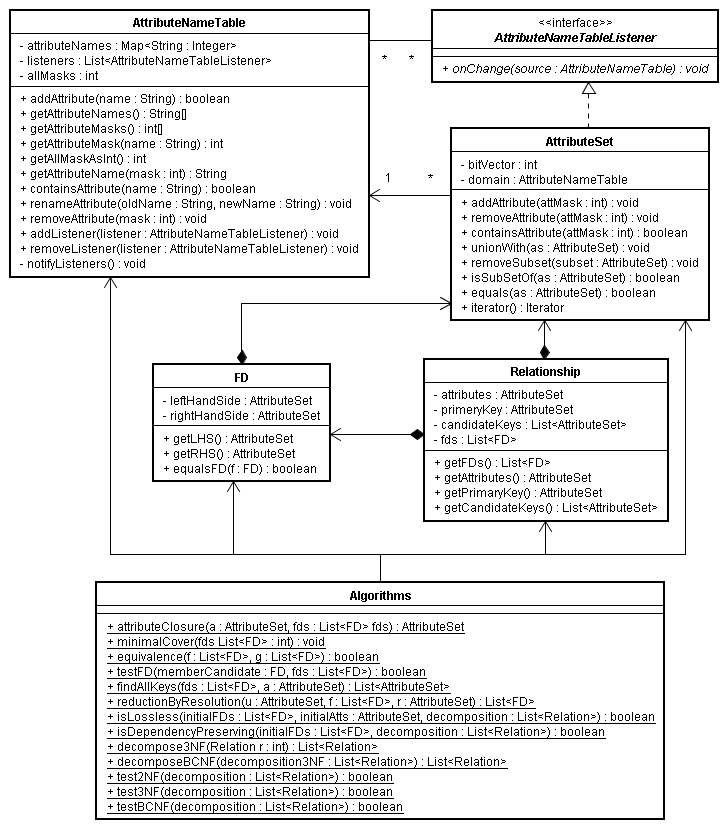
\includegraphics[width=1.08\textwidth]{./img/uml-std.png}
%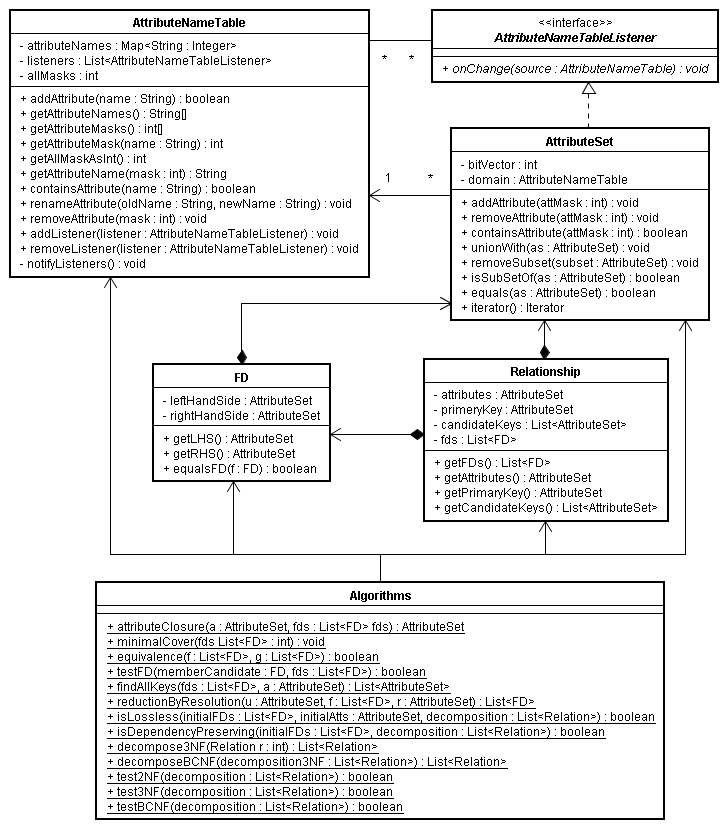
\includegraphics[width=1.00\textwidth]{./img/uml-std.png}
    \caption{UML Class Diagram of LDBN's Core Classes}
    \label{fig:coreuml}
  \end{center}
\end{figure}

%%%%%%%%%%%%%%%%%%%%%%%%%%%%%%%%%%%
% Algorithms                      %
%%%%%%%%%%%%%%%%%%%%%%%%%%%%%%%%%%%
\section{Normalization Algorithms}
\label{sec:alg}
In this section we present different normalization algorithms which are used
in LDBN. A proof of their correctness and complexity would be out of the 
scope of this report and therefore it is omitted. We provide the
reader with textual description and/or pseudo code for each algorithm. 
A reference to additional information is also given. However, in this section we do not
illustrate how the algorithms are applied in the learning environment in order
to perform the \textit{Solve Assignment} and the \textit{Check Solution} functions.
This is done in Section~\ref{sec:keyfunctions}.

We can divide the normalization algorithms used by LDBN into two different groups:

\begin{enumerate}
  \item \textit{Algorithms for Testing} are used to test whether a relation is satisfying a certain normal form criteria.
  \item \textit{Decomposition Algorithms} are used to automatically decompose a relation into a certain normal form.
\end{enumerate}

\subsection{Algorithms for Testing}
\label{sec:algtest}
As we mention earlier we need algorithms for testing whether a decomposition 
is in 2NF, 3NF and BCNF, since a given schema may have many decompositions into a given normal form. Therefore,
simply computing one such decomposition with the \textit{Decomposition Algorithms} and comparing the student's solution to it is
not satisfactory. 

In this section we introduce algorithms for testing weather a decomposition 
is satisfying the lossless-join property, the
dependency preservation property, the 2NF, 3NF and BCNF properties. 
However, most of these algorithms depend on other, more general
algorithms, which we present first.  

\subsubsection{Attribute Closure}
Let $\alpha$  be a set of attributes. 
We call the set of attributes determined by $\alpha$ under a set $F$ of 
FDs the closure of $\alpha$ under $F$, denoted $\alpha +$. The following algorithm
computes $\alpha+$

\begin{alltt}
INPUT
  \(\alpha\)  : a set of attributes
  \(F\)  : a set of FDs
OUTPUT
  \(\alpha+\) : a complete set of attributes  \(\alpha+\)  with  \(\alpha \rightarrow \alpha+\)
BEGIN
  \(\alpha+ = \alpha\)
  while(No more changes in \(\alpha+\)) do
    foreach FD \(\beta \rightarrow \gamma\) in \(F\) do
      if \(\beta \subseteq \alpha+\) then \(\alpha+ \cup \gamma\)
    return \(\alpha+\)
\end{alltt} 

The \textit{Attribute Closure} algorithm is one of the most important algorithms used in LDBN. It is
part of every other normalization algorithm in the system. Therefore every improvement 
of the algorithm is significant. 
The above algorithm is described in many textbooks including~\cite{bdb1, bdb2, bdb4}.
It has worst case behavior quadratic in the size of $F$ and
it is not suitable for large application like LDBN. We presented it only because it is
easy to follow. In our learning environment we use a linear but more complicated algorithm for computing $\alpha+$ 
called $SL_{FD}-Closure$~\cite{p10}:

\begin{alltt}
INPUT
  \(\alpha\)  : a set of attributes
  \(F\)  : a set of FDs
OUTPUT
  \(\alpha+\) : a complete set of attributes  \(\alpha+\)  with  \(\alpha \rightarrow \alpha+\)
BEGIN
  \(\alpha\sb{new} = \alpha\)
  \(\alpha\sb{old} = \alpha\)
  repeat
    foreach FD \(\beta \rightarrow \gamma\) in \(F\) do
      if \(\beta \subseteq \alpha\sb{new}\) then 
        \(\alpha\sb{new} \cup \gamma\)
        \(F = F - \{\beta \rightarrow \gamma\}\) 
      elsif \(\gamma \subseteq \alpha\sb{new}\) then
        \(F = F - \{\beta \rightarrow \gamma\}\) 
      else
        \(F = F - \{\beta \rightarrow \gamma\}\) 
        \(F = F \cup \{\beta-\alpha\sb{new} \rightarrow \gamma-\alpha\sb{new}\}\) 
      end if
    end foreach 
  until ((\(\alpha\sb{new} = \alpha\sb{old}\)) or \(|F| = 0\))
  return \(\alpha+ = \alpha\sb{new}\)
\end{alltt} 

There are several direct uses of the \textit{Attribute Closure} algorithm~\cite{bdb4}:
\begin{description}
    \item[Superkey Test:] To test whether $\alpha$ is a superkey, we compute $\alpha+$, and check whether $\alpha+$ contains all attributes of $R$.
    \item[Computing F+:] For each $\gamma \subseteq R$ we find the closure $\gamma+$, and for each $S \subseteq \gamma+$, we output a FD $\gamma \rightarrow S$.
\end{description}

\subsubsection{FD Test}
To check whether a functional dependency $\alpha \rightarrow \beta $ 
holds (i.e. is in $F+$), just check whether $\beta \subseteq \alpha+$ holds~\cite{bdb4}.
 
\begin{alltt}
INPUT 
  \(f\) : a FD of the form \(\alpha \rightarrow \beta\)
  \(F\) : a set of FDs
OUTPUT 
  true if \(f \in F+\), false otherwise
BEGIN
  compute \(\alpha+ = AttributeClosure(\alpha, F)\)   
  if \(\beta \in \alpha+\) then
    return true
  else
    return false
\end{alltt}
  
\subsubsection{Equivalence}
To determine whether two set of FDs $F$ and $G$ are equivalent, we need to prove that $F+ = G+$. 
However, computing $F+$ or
$G+$ is exponential, therefore this approach cannot be recommended for practical use.
Fortunately, there is a much faster algorithm. We can conclude that $F$ and $G$ are
equivalent, if we can prove that all FDs in $F$ can be inferred from the set of FDs in $G$ and vice
versa. To achieve this we use the \textit{FD Test} algorithm.

\begin{alltt}
INPUT 
  \(F\) : a set of FDs
  \(G\) : a set of FDs
OUTPUT 
  true if \(F \equiv G\), false otherwise
BEGIN
  foreach FD \(f : \alpha \rightarrow \beta\) in \(F\) do
    if not \(FDTest(f, G\)) then
      return false
  end foreach
  
  foreach FD \(g : \alpha \rightarrow \beta\) in \(G\) do
    if not \(FDTest(g, F\)) then
      return false
  end foreach
  
  return true
\end{alltt}

\subsubsection{Lossless-Join Property Test}
In Section~\ref{sec:decofrel} it was shown that a decomposition of $R$ into $R_1$ and $R_2$ 
has a lossless-join if one of the following FDs is in $F+$
\begin{itemize}
  \item $f : R_1 \cap R_2 \rightarrow R_1$ 
  \item $g : R_1 \cap R_2 \rightarrow R_2$ 
\end{itemize}

We can use the \textit{FD Check} algorithm to test whether $f$ or $g$ are in $F+$. Furthermore,
in~\cite{bdb2}, Section~6.5.1, it has been shown inductively that the above rule can be applied for a 
decomposition with $n$ subschemas by using the associativity of the natural join~($\Join$):
$$
  R_1 \Join (R_2 \Join (...\Join(R_{n-1} \Join R_{n}) \newline
  =R_1 \Join (R_2 \Join (...\Join(R_{n-2} \Join R_{n-1}')  \newline
  =
  ...
  = R
$$
Knowing these facts, we can now define a simple algorithm for testing the lossless-join
property of a decomposition \(\mathcal{R}\):
   
\begin{alltt}
INPUT 
  \(R\) : a relation
  \(F\) : a set of FDs which hold in \(R\)
  \(\mathcal{R}\) : a set of relations representing a decomposition of \(R\).
OUTPUT 
  true if  \(\mathcal{R}\) is lossless-join, false otherwise
BEGIN
  K = first element of \(\mathcal{R}\)
  foreach \(R\sb{i} \in \mathcal{R}\) for \(i \geq 2\) do
    if \(FDCheck(K \cap R\sb{i} \rightarrow K, F)\) or \(FDCheck(K \cap R\sb{i} \rightarrow R\sb{i}, F)\) then
      \(K = K \cup R\sb{i}\)
    else
      return false
    end if
  end foreach
  return true
\end{alltt}

%In the above algorithm we are using the $\cup$ operator instead of $\Join$. This is
%permitted, since we are using only the attributes of the relation $R$ and not actual instances (i.e.,
%relation with its contents).

\subsubsection{Dependency Preservation Test} 
Using the \textit{Equivalence} algorithm testing whether a decomposition $R_1,...,R_n$ of $R$ is dependency preserving
becomes quite an easy task. We just need to compute: $$Equivalence(F, (F_1 \cup ... \cup F_n)) \mbox{ where } F_i \mbox{ is the set of FDs which holds in } R_i$$ 

\subsubsection{Find All Candidate Keys}
The problem of finding all candidate keys is know to be NP-complete~\cite{p3}. 
Our leaning environment uses an trivial algorithm for finding all the candidate keys,
which is based on the \textit{Attribute Closure} algorithm. The algorithm test every possible
subset of attributes of the relation for being a superkey. If a subset of the superkey
is found which is also a superkey, then the first superkey is replace with the new one.   

\begin{alltt}
INPUT 
  \(R\) : a relation
  \(F\) : a set of FDs which hold in \(R\)
OUTPUT 
  \(\mathcal{K}\) : a set of all candidate keys for \(R\)
BEGIN
  \(\mathcal{K} = \emptyset\)
  foreach subset \(\gamma\) of \(R\) do
    compute \(\gamma+\)
    if \(\gamma+ \) contains all attributes of \(R\) then
      remove all \(\kappa \in \mathcal{K}\) with  \(\gamma \subseteq \kappa\)
      if \(\gamma \nsubseteq \kappa\) for all \(\kappa \in \mathcal{K}\) then
        \(\mathcal{K} \cup \gamma\)
      end if
    end if
  end foreach
return \(\mathcal{K}\)
\end{alltt}

\subsubsection{Reduction By Resolution}
Often is required to compute a cover for the projection of $F$ on a subschema $X$ of $R$, in 
other words, to find find the FDs on $R$ which are induced by $F$. Altought the problem of
finding such embedded cover of FDs is
known to be inherently exponential~\cite{p11}, it plays an important part of many of the algorithms
used by LDBN. The traditional approach is to compute $F+$ and then project $F+$ over the subschema $X$,
however, the produced cover
is always unnecessarily large~\cite{p4}. Still, for this difficult problem a simple 
algorithm called \textit{Reduction by Resolution}
was found by Gottlob~\cite{p4}. The algorithm is much more practical than the standard approach,
as it runs in polynomial time in a large number of cases, unlike the standard approach
which is exponential for each input. 

\begin{alltt}
INPUT 
  \(R\) : a relation
  \(F\) : a set of FDs which hold in \(R\)
  \(X\) : a subset of attributes of \(R\)
OUTPUT 
  \(F\sb{X}\) : a cover for \(F\sb{X}+\) with 
           \(F\sb{X}+ = \{\alpha\rightarrow\beta | \alpha \rightarrow \beta \in F+ \wedge \alpha \subseteq R \wedge \beta \subseteq R\}\)
BEGIN 
  \(G = F\)
  \(K = X - R\)
  while \(K \neq \emptyset\) do
    choose an element \(A \in K\),
    \(K = K - A\),
    \(RES = \emptyset\)
    foreach FD \(f\) in \(F\) of the form \(Y \rightarrow A\) do
      foreach FD \(g\) in \(G\) of the form \(AZ \rightarrow B\) do
        \(h = YZ \rightarrow B\),
        /* h is the resolvent of f and g */
        if h not trivial then \(RES = RES \cup \{h\}\)
      end foreach
    end foreach
    foreach FD \(f\) in \(G\) do
      if \(A\) occurs in \(f\) then \(G = G - \{f\}\)
    end foreach
    \(G = G \cup RES\)
  end while
  return \(G\)
\end{alltt}

\subsubsection{BCNF Test}
To check whether a non-trivial dependency $\alpha \rightarrow \beta$  causes a violation of BCNF,
we must use the \textit{Attribute Closure} to test whether $\alpha$ is a superkey. 
It suffices to check only the dependencies in the given set $F$ for violation of BCNF, 
rather than checking all dependencies in $F+$~\cite{bdb4}.  
If none of the dependencies in $F$ causes a violation of BCNF, 
then none of the dependencies in $F+$ will cause a violation of BCNF either.
However, using only $F$ is incorrect when testing a relation in a decomposition of $R$~\cite{bdb4}.
Let us consider the following example:

\begin{center}
\begin{tabular}[h]{l l}
  $R = \{A, B, C, D, E\}$ & $F = \{A \rightarrow B, BC \rightarrow D\}$ \\
  Decompose $R$ in:  & $R_1 = \{A, B\} \mbox{ and } R_2 = \{A, C, D, E\}$ \\ 
\end{tabular}
\end{center}

Neither of the dependencies in $F$ contain only attributes from
$(A,C,D,E)$ so we might be mislead into thinking $R_2$ satisfies BCNF. In fact, 
dependency $AC \rightarrow D$ in $F+$ shows $R_2$ is not in BCNF. To avoid this we can
use the \textit{Reduction by Resolution} algorithm to compute covers for $R_1$ and $R_2$. 

The algorithm uses the \textit{Reduction by Resolution} algorithm which is know to be exponential
in some bad cases, thus the \textit{BCNF Test} is also exponential. In fact, the test is know to 
be co-NP-complete~\cite{p4}.

\subsubsection{3NF Test}
The \textit{3NF Test} is similar to the \textit{BCNF Test}. By using the \textit{Reduction by Resolution} algorithm
we must first compute the
embedded FD cover $F_i$ for each relation $R_i$ in a decomposition $R_1,...,R_n$ of $R$. Then we use 
the \textit{Attribute Closure} to test each FD in $F_i$ of the form $\alpha \rightarrow \beta$ 
whether $\alpha$ is a superkey in $R_i$. 
If the $\alpha$ is not a superkey, we have to verify whether each attribute in the $\beta$ 
is contained in a candidate key of $R$, i.e., it is prime. Testing attribute for being a prime
attribute is know to be a NP-complete problem~\cite{p3}. For this part of the \textit{3NF Test} algorithm
we can use our \textit{Find All Candidate Keys} algorithm in order
to compute all the candidate keys in $R_i$ and then test whether the attributes in $\alpha$ are part of any 
of them.

\subsubsection{2NF Test}
%Testing whether a a decomposition is in 2NF is even harder than the \textit{3NF Test}. 
Once again we compute the
embedded FD cover for each relation $R_i$ in a decomposition $R_1,...,R_n$ of $R$. After that 
we compute each candidate key for each for each a relation $R_i$, we refer to this set as $K_i$.
 
To test whether $R_i$ is in 2NF we have to ensure that each non-key attribute is fully
functional dependent on every candidate key in $K_i$. To simply the problem we can test
each FD in $F_i$ of the form $\alpha \rightarrow \beta$ whether $\alpha$ is a proper subset
of a key candidate in $K_i$. If this is true and the attributes in $\beta$ are not prime then
$R_i$ is not in 2NF.

The \textit{2NF Test} is NP-complete, since it involves finding all candidate keys.

\subsection{Decomposition Algorithms}
\label{sec:algdec}
In previous sections we already decomposed some relations without
a formal definition of the rules which we were following during this process. 
In this section we present algorithms for finding a minimal cover of a set of FDs and 
for decomposing any proposed relation into 3NF and BCNF.  

\subsubsection{Find Minimal Cover}
With the help of the \textit{Attribute Closure} algorithm we can now define an algorithm 
for computing a minimal (canonical) cover of a set $F$ of FDs. The algorithm comes form~\cite{bdb2}, Section~6.3.1.

\begin{alltt}
INPUT 
  \(F\)  : a set of FDs
OUTPUT 
  \(F\sb{c}\) : a minimal (canonical) cover of \(F\)
BEGIN

\(F\sb{c} = F\)
repeat
  /* Find redundant attributes in the left-hand side of each FD */
  foreach FD \(\alpha \rightarrow \beta\) in \(F\sb{c}\) do
    foreach \(A \in \alpha\) do
      /* Checks if A is redundant */
      if \(\beta \subseteq AttributeClosure(F\sb{c}, \alpha-A)\) then
        replace \(\alpha \rightarrow \beta\) with \((\alpha-A) \rightarrow \beta\)
      end if
    end foreach
  end foreach
    
  /* Find redundant attributes in the right-hand side of each FD */
  foreach FD \(\alpha \rightarrow \beta\) in \(F\sb{c}\) do
    foreach \(B \in \beta\) do
      /* Checks if B is redundant */
      if \(B \subseteq AttributeClosure(F\sb{c}-(\alpha \rightarrow \beta) \cup (\alpha \rightarrow (\beta - B)), \alpha)\) then
        replace \(\alpha \rightarrow \beta\) with \((\alpha \rightarrow (\beta-B)\)
      end if
    end foreach
  end foreach
    
  Delete all FDs FD of the form \(\alpha \rightarrow \emptyset\) form \(F\sb{c}\)
    
  Using the \(Union Rule\) combine all FDs of the form \(\alpha \rightarrow \beta,...,\alpha \rightarrow \gamma\)
    into one FD \(\alpha \rightarrow (\beta \cup ... \cup \gamma)\)
    
until \(F\sb{c}\) does not change
return \(F\sb{c}\)
\end{alltt}

For the sake of simplicity we iterate over all FDs in $F$ several times, in the actual implementation
the number of iteration could be reduced. 

\subsubsection{3NF Decomposition}
The following algorithm decomposes a relation schema in 3NF. The algorithm
ensures that each new relation schema is in 3NF, thus the decomposition is in 3NF. 
Furthermore, the decomposition is dependency preserving and lossless-join. 
The algorithm comes form~\cite{bdb2}, Section~6.8. 
First, we build new relations corresponding to each FD in in $F_{c}$ (the minimal cover of $F$). 
Then we need to eliminate relations, the attributes of
which are subset of the attributes of another relation. 
After that, we find all the candidate keys of
the initial relation, this is necessary in order to determine  whether one of them is present
in the new set of relations, which is required by the algorithm to ensure
dependency preservation. If this is not the case, the algorithm creates
a new relation \(\mathcal{R}\sb{i}\) = any candidate key for \(R\).
Here follows a pseudo code of the algorithm:

\begin{alltt}
INPUT 
  \(R\)  : a relation
  \(F\sb{c}\) : a canonical cover of a set of FDs which hold in \(R\)
OUTPUT 
  \(\mathcal{R}\) : a set of relational schemas representing a decomposition in 3NF 
BEGIN
  \(\mathcal{R} = \emptyset\)
  i = 0
  foreach FD \(\alpha \rightarrow \beta\) in \(F\sb{c}\) do
    i = i + 1
    create a relation schema \(\mathcal{R}\sb{i} = \alpha \cup \beta\)
    assign \(\mathcal{R}\sb{i}\) the FDs  \(F\sb{i} = \{\alpha\sp{'} \rightarrow \beta\sp{'} \in F\sb{c}\ | \alpha\sp{'} \cup \beta\sp{'} \subseteq \mathcal{R}\sb{i}\}\)
    \(\mathcal{R} = \mathcal{R} \cup \mathcal{R}\sb{i}\)
  end foreach
  
  if none of the schemas \(\mathcal{R}\sb{j}, 1 \leq j \leq i\) contains a candidate key for \(R\) then
    i = i + 1
    create a relation schema \(\mathcal{R}\sb{i}\) = any candidate key for \(R\)
    \(\mathcal{R} = \mathcal{R} \cup \mathcal{R}\sb{i}\)
    
  Delete all relational schemas \(\mathcal{R}\sb{a}\) from \(\mathcal{R}\) with \(\mathcal{R}\sb{a} \subseteq \mathcal{R}\sb{j},  1 \leq j \leq i\)
  
  return \(\mathcal{R}\)
\end{alltt}

\subsubsection{BCNF Decomposition}
There is a simple algorithm for decomposing a relational schema into BCNF.
It is described in~\cite{bdb2}, Section~6.9:

\begin{alltt}
INPUT
  \(R\) : a relation
  \(F\) : a set of FDs which hold in \(R\)
OUTPUT
  \(Z\) : a set of relational schemas representing a decomposition in BCNF 
BEGIN
\(Z = R\)
done = false

while not done do
  if there is a schema \(R\sb{i}\) in \(Z\)  that is not in BCNF then begin
    let \(\alpha \rightarrow \beta\) be a nontrivial FD that holds on \(R\sb{i}\)
      such that \(\alpha \nrightarrow R\sb{i}\) /* \(\alpha\) is not a superkey */
      and  \(\alpha \cap \beta \neq \emptyset\) then  
        decompose \(R\sb{i}\) in \(R\sb{i1} = \alpha \cup \beta\) and \(R\sb{i2} = R\sb{i} - \beta\)
        remove \(R\sb{i}\) from \(Z\) 
        \(Z = Z \cup R\sb{i1} \cup R\sb{i2}\)
  else 
    done = true
  end if 
return \(Z\)
\end{alltt}

The algorithm always 
procures a lossless-join decomposition, however, we must run the \textit{Dependency Preservation Test} on
the decomposition to check whether the decomposition is dependency preserving or not. As we mention in Section~\ref{sec:BCNF},
it is no always possible to find a dependency preserving BCNF decomposition.



\section{Key Functions of LDBN}
\label{sec:keyfunctions}
As we stated earlier, the two most important functions of LDBN are the \textit{Solve Assignment} and 
the \textit{Check Solution} functions. They build the foundation of the system and
without them UI will lose its purpose. Therefore, we
discuss the two function more formally in this section.

\subsubsection{Solve Assignment}  
The \textit{Solve Assignment} function can provide the user with a sample solution
to an assignment, thus it decomposes a database schema from URF into 3NF and BCNF. This
task involves several algorithms. Figure~\ref{fig:orderdecomposition} is 
illustrates the order in which those algorithms are applied.

\begin{figure}[h]
	\begin{center}
		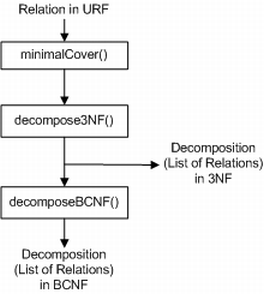
\includegraphics[scale=0.6]{./img/decomposition1a.png}
		\caption{Order of the Decomposition Algorithms}
		\label{fig:orderdecomposition}
	\end{center}
\end{figure}

First, the schema is passed trough the
\verb=minimalCover()= method of the \verb=Algorithms= class, which
implements the Algorithm \textit{FindMinimalCover} of Figure~\ref{alg:mincov}. 
After that we use the \verb=decompose3NF()= method, which implements the 
decomposition algorithm described in Figure~\ref{alg:dec3nf}. 
We use the new decomposition also as a solution for the 2NF, since
a decomposition in 3NF is also in 2NF. 

For computing the BCNF decomposition we use 
a slight modification of the Algorithm \textit{DecompositionBCNF} of Figure~\ref{alg:decbcnf}.
In our implementation
the input for the algorithm is not the initial schema in URF, but the decomposition
produced by the \verb=decompose3NF()= method. By doing this we 
increase the performance of the system, since many decompositions which 
are in 3NF are also in BCNF, or the differences are usually rather small, thus the algorithm
requires fewer passes.   
  
A given schema will always have a dependency-preserving 3NF
decomposition, as well as a BCNF decomposition, but not necessarily a
dependency-preserving BCNF decomposition. Thus, there are two
distinct final goals for decomposition which may not always be
realizable simultaneously. Because of this fact, we do not present the BCNF decomposition as solution
for the 3NF, even though BCNF decompositions are also in 3NF.

\subsubsection{Check Solution}  
The \textit{Check Solution} function of LDBN allows the system to test a solution 
provided by the user and assess its correctness relative to many factors, which
we present later in this section. As we mentioned earlier it is not possible
to compare a solution produces by LDBN to the one of the user, since there may be many
possible solutions/decompositions to a given database schema. Therefore we need the
algorithms for testing a decomposition described in Section~\ref{sec:algtest}. In this section
we illustrate how we apply those algorithms in our implementation. 

First of all, a solution in LDBN is represented as a list of instances of the
\verb=Relation= class. Those objects are built from the user input. The list is then
passed to the static functions in the \verb=Algorithm= class, which 
implement the all of the algorithms described in Section~\ref{sec:alg}. 
The system analyzes the solution to the following factors:

\begin{description}
  \item [Correctness of the FDs] of each relation, this means, testing whether the FDs associated by the user
    for each new relation are actually in the closure of FDs for this relation. We do this by
    using the Algorithm \textit{ReductionByResolution} of Figure~\ref{alg:rbr} for computing the embedded closure of FDs for the given
    relation. This algorithm is implemented by the \verb=reductionByResolution()= method. Then we apply
    the \textit{Equivalence} algorithm of Figute~\ref{alg:equivalence}, to test 
    whether both set of FDs, the one produced by 
    the algorithm and the one provided by the user, are equivalent. Here the Algorithm \textit{ReductionByResolution}
    can have exponential complexity in some bad cases~\cite{p4}, therefore we cache the results
    of the algorithm for future use, e.g., when the user needs to recheck his solution, which can happen
    quite often during the process of solving an assignment correctly. 

	\item [The Losses Join] properly for every decomposition. This check is done by directly applying the 
		Algorithm \textit{TestLosslessJoin} of Figure~\ref{alg:lossless}, which is 
		implemented by the \verb=isLossless()= method.
		
	\item [Dependency Preservation] for every decomposition. This check is done by directly applying the 
		Algorithm \textit{TestDependencyPreservation} of Figure~\ref{fig:dptest}, which is implemented by the 
		\verb=isDependencyPreserving()= method.
		
	\item [Correctness of the Key] of each relation. This check is performed by first computing 
		every possible candidate key 
		for each new relation, by applying the Algorithm \textit{FindAllCandidateKeys} of Figure~\ref{alg:findkeys}, 
		which is implemented
		by the \verb=findAllKeys()= method. The method returns a list of all possible candidate keys
		for a given relation. Then the system searches if the key suggested by the user is 
		present in that list. The algorithm is quite slow due to the fact that the problem of
		finding all candidate keys is know to be NP-complete~\cite{p3}. To improve performance LDBN
		caches every list found for each relation, so that whenever a user needs to rechecks his/her solution
		the system computes only the lists of candidate keys for new, uncached relations.  
		
	\item [Correctness of the Decomposition] In this check we apply directly the 
		\textit{Test2NF, Test3NF, Test BCNF}, which are implemented by the 
		\verb=test2NF()=, \verb=test3NF()=, \verb=testBCNF()= methods.
\end{description}

All the checks are performed in the exact order described above. If one of the checks fails the following ones
are not executed. This way we are able to give the user faster feedback, because 
the most computationally expensive checks are at the end. For example, if the \textit{Dependency Preservation}
check, which is performed in polynomial time, fails, then the other check such as the 
\textit{Correctness of the Key} and the \textit{Correctness of the Decomposition}, both of which 
have exponential complexity, are omitted, thus the user could get a much faster response from the system
in case of an error. 

\section{User Interface}
The most important part of a system for end users and critical for system 
success is the user interface (UI)~\cite{p9}, as such we put most of
our efforts in developing a fast, intuitive and stable UI. Furthermore,
it is possible to define two distinct user groups, warranting at least two different
user interfaces for LDBN.  One group would include the lecturers, who will
focus their attention on creating assignments. The other group would be the 
students, who will use the leaning environment mostly for solving 
the assignments provided by the lecturers. It should be noted that every registered
user can create assignments, thus students can take the role of lecturers as well.
We tried to provide both 
user groups with fast and easy to use UI. In order to achieve this we put a lot
of our attention in finding a good layout for the UI. The requirements for
the layout were to give the user as much information possible about an 
assignment without losing the general view. In order to achieve this goal  
we split the UI in four different views using tabs:

\begin{description}
	\item[Home] view is where the users can login, register and view some information 
	about the learning environment. It can be seen in Figure~\ref{fig:hv}.
	\item[Solve Assignment] view is where students can load an assignment, give and
	test their solutions. In case they have troubles finding a correct solution
	LDBN could generate a sample one and present it. Figure~\ref{fig:sav} is showing
	the view with a loaded assignment.
	\item[Create Assignment] view is used by lecturers to create, edit, export or import
	assignments. It can be seen in Figure~\ref{fig:cav}.
	\item[License] view displays a license information about LDBN.
\end{description} 

\begin{figure}[h]
	\begin{center}
		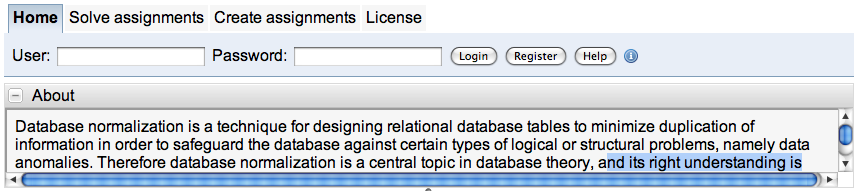
\includegraphics[width=0.85\textwidth]{./img/screen-tab1.png}
		\caption{Home View}
		\label{fig:hv}
	\end{center}
\end{figure}

\begin{figure}[h]
	\begin{center}
		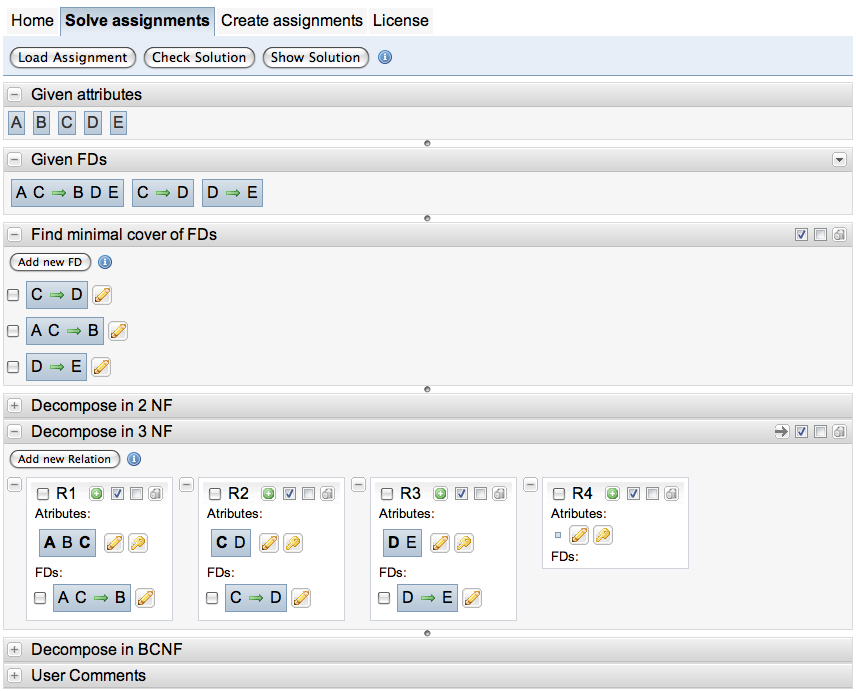
\includegraphics[width=0.85\textwidth]{./img/screen-tab2.png}
		\caption{Solve Assignments View}
		\label{fig:sav}
	\end{center}
\end{figure}

\begin{figure}[h]
	\begin{center}
		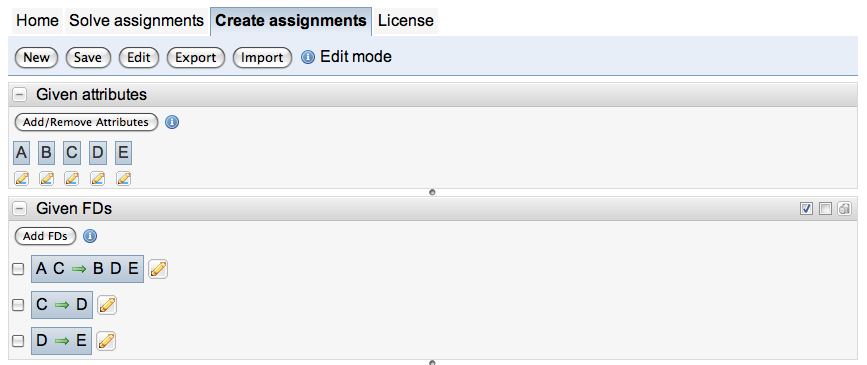
\includegraphics[width=0.85\textwidth]{./img/screen-tab3.png}
		\caption{Create Assignments View}
		\label{fig:cav}
	\end{center}
\end{figure}


\subsubsection{Solve Assignment View}
The most important view for students is definitely the \textit{Solve Assignment} view.
It contains the following fields:

\begin{itemize}
	\item Given attributes.
	\item Given FDs.
	\item Minimal Cover.
	\item 2NF, 3NF, BCNF Decomposition.
	\item Comments.
\end{itemize}

The \textit{Given Attitibutes} and the \textit{Given FDs} fields are not editable
and they correspond	to the information stored in each assignment, which is all the 
attributes and all the FDs of a database schema in URF. In all other fields 
the content can be modified by the user using different editors,
such as the \textit{Attribute Editor} (Figure~\ref{fig:attedit}), 
the \textit{Key Editor} (Figure~\ref{fig:keyedit}) and the \textit{FD Editor}
(Figure~\ref{fig:fdedit}).
All of those editors contain one or two text boxes, where users can input 
different attribute names separated by commas
in order to define respectively attributes of a relation, a key or a set of FDs. With
the help of the editors the user can define relations as the one shown on 
Figure~\ref{fig:relui}. In this example we have a relation with attributes 
\textit{\{A, B, C\}}, a key \textit{\{A, C\}} and only one FD in the set of FDs,
namely \textit{\{A, B $\rightarrow$ C\}}.  Furthermore,
each of the editors is wrapped in a draggable dialog window. 
In this way, the editors do not require any space on any of the fields, 
and can be opened only when they are needed. In addition to this, every attribute and every FD,
as the ones shown in the relation on Figure~\ref{fig:relui}, can be dragged and
dropped in the text box of each editor, as a result of which the attributes/FDs
are automatically inserted in the text areas of the editor.
This can help user define attributes, keys or
FDs much more quickly, which on the other hand can help improve the usability of 
the learning environment. 

\begin{figure}[h]
	\centering
	\subfigure[Attribute Editor]{
		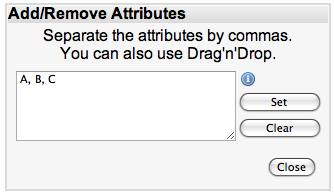
\includegraphics[scale=0.4]{./img/screen-atteditor.png}
		\label{fig:attedit}
	}
	\subfigure[Key Editor]{
		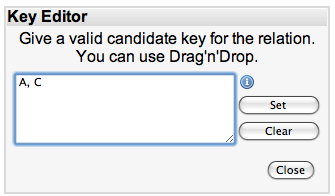
\includegraphics[scale=0.4]{./img/screen-keyeditor.png}
		\label{fig:keyedit}
	}
\caption{Attribute and Key Editor}
\end{figure}

\begin{figure}[h]
	\centering
	\subfigure[FD Editor]{
		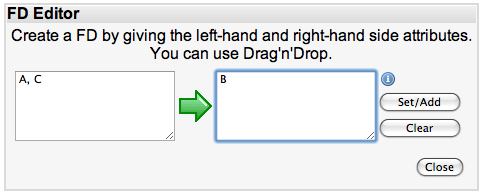
\includegraphics[scale=0.4]{./img/screen-fdeditor.png}
		\label{fig:fdedit}
	}
	\subfigure[Relation]{
		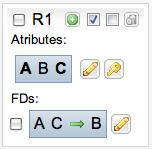
\includegraphics[scale=0.52]{./img/screen-rel.png}
		\label{fig:relui}
	}
\caption{FD Editor and an Example of a Relation in LDBN}
\end{figure}

We continue with the different fields in \textit{Solve Assignment} view. 
The first one is the \textit{Minimal Cover} field, where the user has to define 
a set of FDs using the \textit{FD Editor}. The user defined FDs must
constitute a minimal cover of the \textit{Given FDs}.
This field is intended to be an intermediate step, which will help the user 
find easier a correct decomposition
in the \textit{2NF, 3NF and BCNF Decomposition} fields. Those last three fields all
work the same way, with the only difference that the alogotithms for checking the 
correnctnes of the 
decomposition are not the same.  
In each decomposition field the user must define a set of relations, as the one shown 
in Figure~\ref{fig:relui}. All the relations
within a field represent a decomposition. To check the decomposition the user must
use the \textit{Check Solution} button, 
after that the system analyzes the solution by the criteria described in 
Section~\ref{sec:keyfunctions} and shows a dialog with the result 
as the one in Figure~\ref{fig:screen03} 

Another useful feature, which also improves the usability of LDBN and greatly reduces
the time for defining relations, 
is the ability to 
import entire decompositions from the 2NF into the 3NF field, and from the 
3NF field into the BCNF field. This was done because usually 
the differences between the decompositions are not huge, and each decomposition
can be used as a good staring point for the other ones.	

The last field of the \textit{Solve Assignemtn} view is the \textit{Comment} field, 
where users can view and post textual comments on every assignment.

\subsubsection{Create Assignment View}
The \textit{Create Assignment} view looks very similar to the 
\textit{Solve Assignment} view. It also has a \textit{Given Attributes} and 
\textit{Given FDs} fields. However, in this view these fields
can be edited using the \textit{Attribute Editor} and the \textit{FD Editor}. 
This allows users to define new assignments or modify existing ones. In addition, the view
allows users to save the assignments in the database or to export them as XML
files to the local file system. Importing an assignment form an XML file is also 
possible.  
\newline
Finally, in case the user needs any help with certain aspects of LDBN, the system provides 
help dialogs for every key feature of the UI. The dialogs can be open
using information buttons (
\includegraphics[scale=0.5]{./img/info.png}), which can be
found near every button or in every editor. This way help information is 
visually organized and the user has fast access to it. An example of such help dialog
window is shown in Figure~\ref{fig:screen-help}.

\begin{figure}[h]
	\begin{center}
		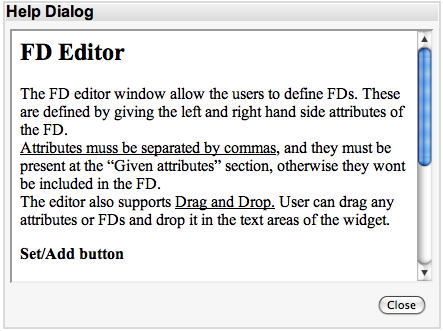
\includegraphics[width=0.5\textwidth]{./img/screen-help.png}
		\caption{Help Dialog for the FD Editor}
		\label{fig:screen-help}
	\end{center}
\end{figure}


\section{Server Side}
The server side is mainly used for persistent storage of assignments, user comments,
user and session data. The communication between the web server and the client
is done using the POST method of the Hypertext Transfer Protocol - HTTP/1.1~\cite{w6}.
The POST method has two advantages over the GET method. First, it is more secure, i.e., 
the GET method is defined as safe, which means it is intended only for information 
retrieval and should not change the state of the server. Second, although the
RFC 2616, "Hypertext Transfer Protocol -- HTTP/1.1"~\cite{w6} does not specify
any requirement for URL length, many browsers such as Internet Explorer limit
the length of an URL to a maximum of 2048 characters. This length may not be 
enough for LDBN, as it sometimes sends very large assignments back to the server.  

The web server uses XML to send data back to the client. LDBN defines its own XML data
exchange format. The format has several types:

\begin{description}
	\item[Message] for sending string messages, which appear in an alert window on 
	the client side. Such messages can be, for instance, an error messages returned
	by the database. 
	\item[Comments] for sending user comments. 
	\item[Session] contains session data for logged in users such as a unique session 
	ID, generated by the server and stored in the database. The ID is used for
	authorizing user actions on the server side.
	\item[Assignment List] for sending back meta data for each assignment. This
	information is used by the \textit{Load Assignment} function in order 
	to display a list of all available assignments from the database.
	\item[Assignment] contains a LDBN assignment. 
\end{description}  

\section{Security Issues}
The system uses HTTP 1.1 for the communication between the client and the web
server. This can easily be secured by using HTTPS instead. The upgrade only
require changes to the configuration of the web server. However, using an encrypted
connection does not prevent web applications from SQL injection and cross-site 
scripting attacks. SQL Injection refers to the technique of 
inserting SQL statements into web-based input fields in 
order to manipulate the execution of the SQL queries. Cross Site Scripting 
attacks work by embedding script tags into the web pages. 

Here follows a short example of a SQL injection.
Assuming that we have a poorly implemented PHP script for loading an assignment,
which has the following line of code in it:

\begin{verbatim}
     $sql_statement := "SELECT * FROM assignment WHERE id=$_GET['id'] ";
\end{verbatim}

\noindent If the $id$ argument of the GET method is crafted in a specific way by a 
malicious user, the SQL statement may do more than the code author intended. 
For example, setting the $id$ argument as:

\begin{verbatim}
     1; DROP TABLE users;
\end{verbatim}

\noindent yields the following SQL statement:

\begin{verbatim}
     SELECT * FROM assignment WHERE id=1; DROP TABLE users;
\end{verbatim}

\noindent The statement would cause the deletion of the $users$ table. 

In order to prevent SQL injection and cross-site 
scripting attacks LDBN uses regular expressions for validating
user input, and it escapes HTML special characters such as \lt and~\gt.
To the best of our knowledge, it is not possible to perform such attacks on LDBN.

Another issue with web-based applications is password protection. LDBN uses the 
MD5~\cite{w7} one-way encryption algorithm for hashing user passwords. 
To authenticate a user, the password presented by him/her is hashed on the client side, 
then send to the web server and compared to the stored hash in the database. 
This way the actual password of the user is never sent over the network.

\chapter{Conclusions}
\label{chap:conclusion}


\chapter{Acknowledgements}
\label{chap:acknowledgements}
I would like to thank my supervisor, Stephen J. Hegner, who has supported me 
throughout my thesis with his patience and knowledge 
while allowing me the room to work in my own way. 
Without him this report would not have been completed.

I would also like to thank Michael H\"ofling for all his help during my stay in Sweden.
Last, and most importantly, I thank my family for their love and support.

%
%In order to use the bibliography{base}-command you have to prepare a "database"
%base.bib in a certain format and then run the bibtex-command (a Unix-command) to create
%a file base.bbl which LaTeX uses to create References
%
\cleardoublepage
\addcontentsline{toc}{chapter}{References}
\renewcommand{\bibname}{References}
\bibliographystyle{plain}
\bibliography{./tex/base}

\appendix
\chapter{Tutorial}
\label{chap:tutorial}
A tutorial to the right usage of LDBN. 
 

\end{document}
